\chapter{Frozen Showers}\label{chap:FS}
\minitoc

\begin{figure}[!b]
\center{
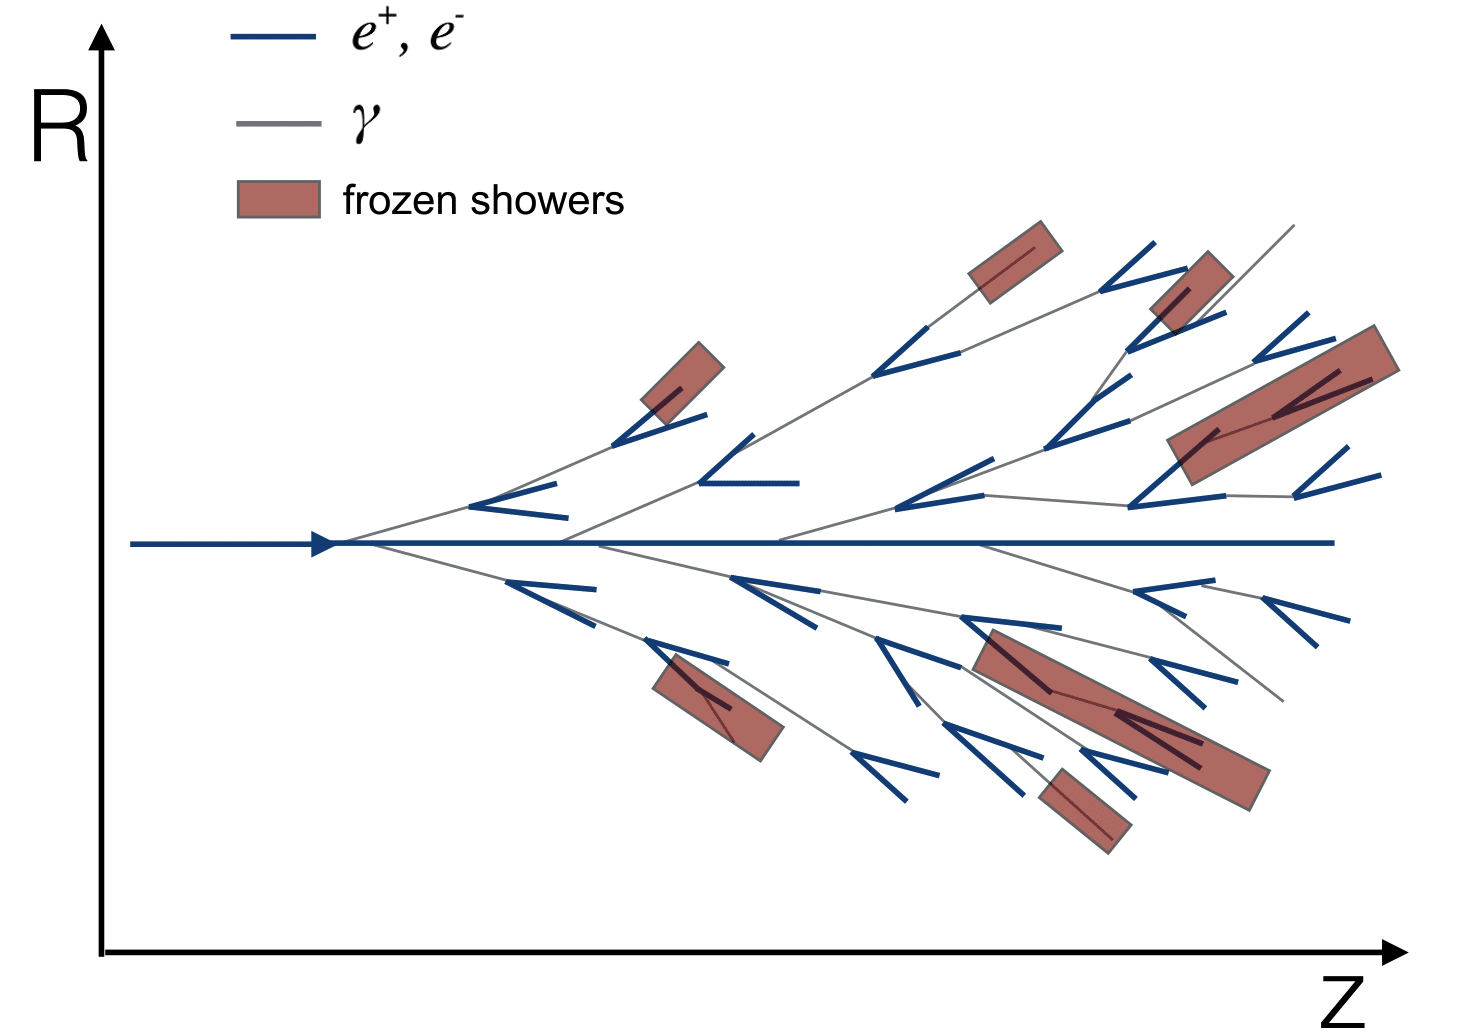
\includegraphics[width=0.7\textwidth]{MC/FSMethod2.png}
\caption{Diagram showing the shower substitution of the low-energy particle, during the high-energy particle simulation. Some of the showers from a particles, substituted by frozen showers method marked by a red squares}
\label{fig:MC_FS_method}
}
\end{figure}
As it was mentioned in a previous chapter, fast simulation techniques are the essential part of Monte-Carlo production at \atlas experiment. Typical time for a simulation of $t\bar{t}$ event is around 1 minute, and most of the time is spend on a simulation of particle interaction in calorimeters. This motivates a development of fast calorimetry techniques. 

Frozen showers is currently the main fast calorimeter simulation approach used at \atlas experiment. In this chapter we will discuss main principles,difficulties and current developments in this method.

Frozen shower method uses pre-simulated "frozen" showers instead of the full simulation. This is allowing to reduce time spend on a simulation of a large amount of low energy sub showers. This method is allowing to have a 25\% speedup in simulation. It is required to have an  in advance generation of a libraries for each detector and particle used in this method. Each shower from a library stores it's lateral and transverse size and list of the all energy depositions inside sensitive material (hits) with information about their energy, position and time. During a simulation, if energy of secondary electron falls below cutoff energy it is replaced by a shower from a library, as shown on a Fig. ~\ref{fig:MC_FS_method}. Main parameters used in \atlas simulation are summarized in a Tab. ~\ref{tab:MC_FS_params}.

\begin{table}[!tbp]
\caption{Main parameters used for the frozen shower libraries}
\label{tab:MC_FS_params}
\centering
\begin{tabular}{l|r}
\hline
\hline
\multicolumn{2}{c}{The general frozen showers parameters} \\
\hline
Detectors used            & FCAL1, FCAL2\\
Type of the particle      & photons, electrons, neutrons \\
Energy range              &  $E_{\gamma}<10$~MeV,  $E_{e}<1000$~MeV,  $T_n<100$~MeV \\
\hline
\end{tabular}

\end{table}



\begin{figure}[!b]
\begin{minipage}[h]{0.49\linewidth}
\center{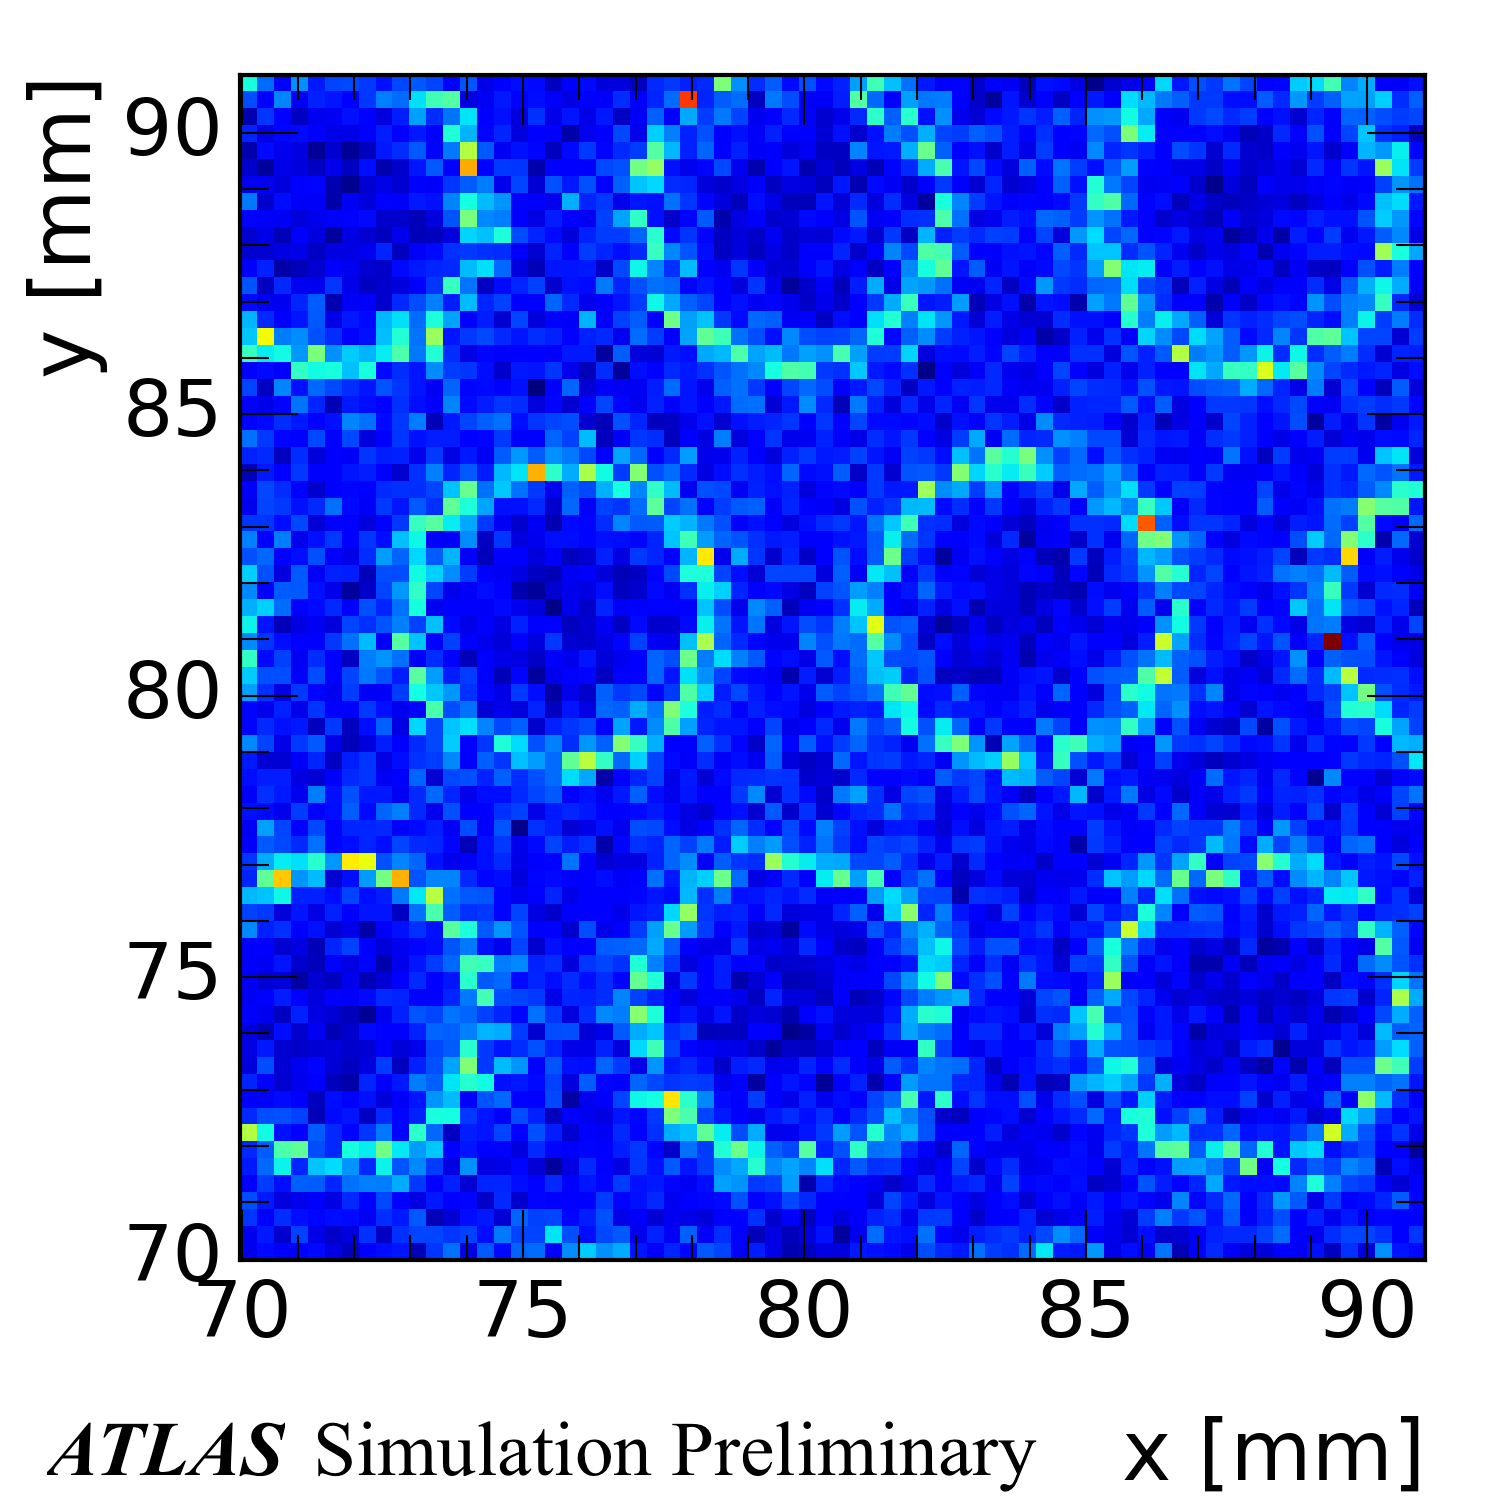
\includegraphics[width=0.9\linewidth]{MC/xySumE.png} \\ a)}
\end{minipage}
\hfill
\begin{minipage}[h]{0.49\linewidth}
\center{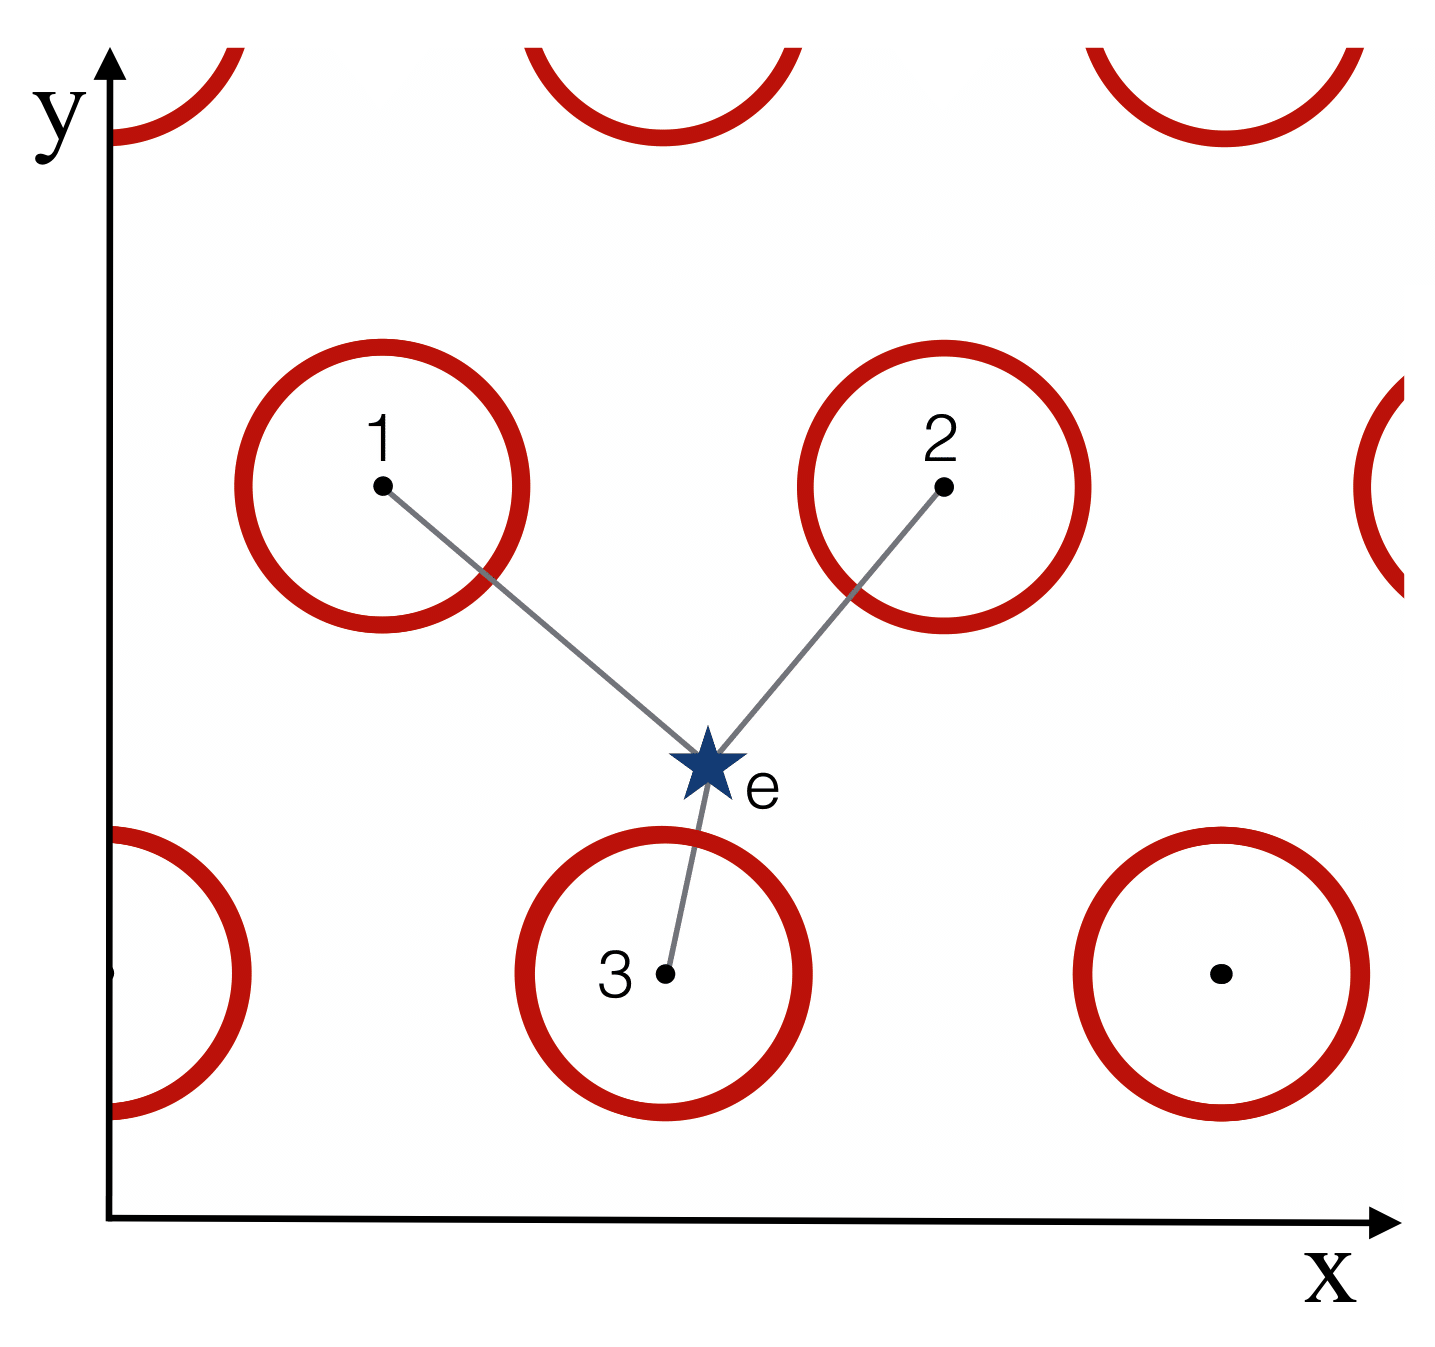
\includegraphics[width=0.9\linewidth]{MC/DistanceCalculation.png} \\b)}
\end{minipage}
\caption{ a) Shower energy response histogram in the x vs y plane for electrons, generated with uniformly distributed x and y and energy less than 1 GeV. Light circles are corresponding to a showers, started inside a LAr gaps with on average higher energy response, while the dark parts are corresponding to dead material respectively with smaller sum of the "hits" energy.
b) Distance to a closest rod center scheme, where $d_{rod} = min( d(1,e), d(2, e), d(3, e))$. Rod centers and liquid argon gaps are shown by black and red circles respectivelly.}
%\caption{Distribution a) electron energies and b) mean number of hits in a shower vs energy of electron for electrons with energy less than 1 GeV coming from initial electron with energy 1 TeV. }
\label{fig:FSFluctuations}
\end{figure}



\section{Problem description}\label{sec:FSproblem}




%\begin{figure}[!b]
%\center{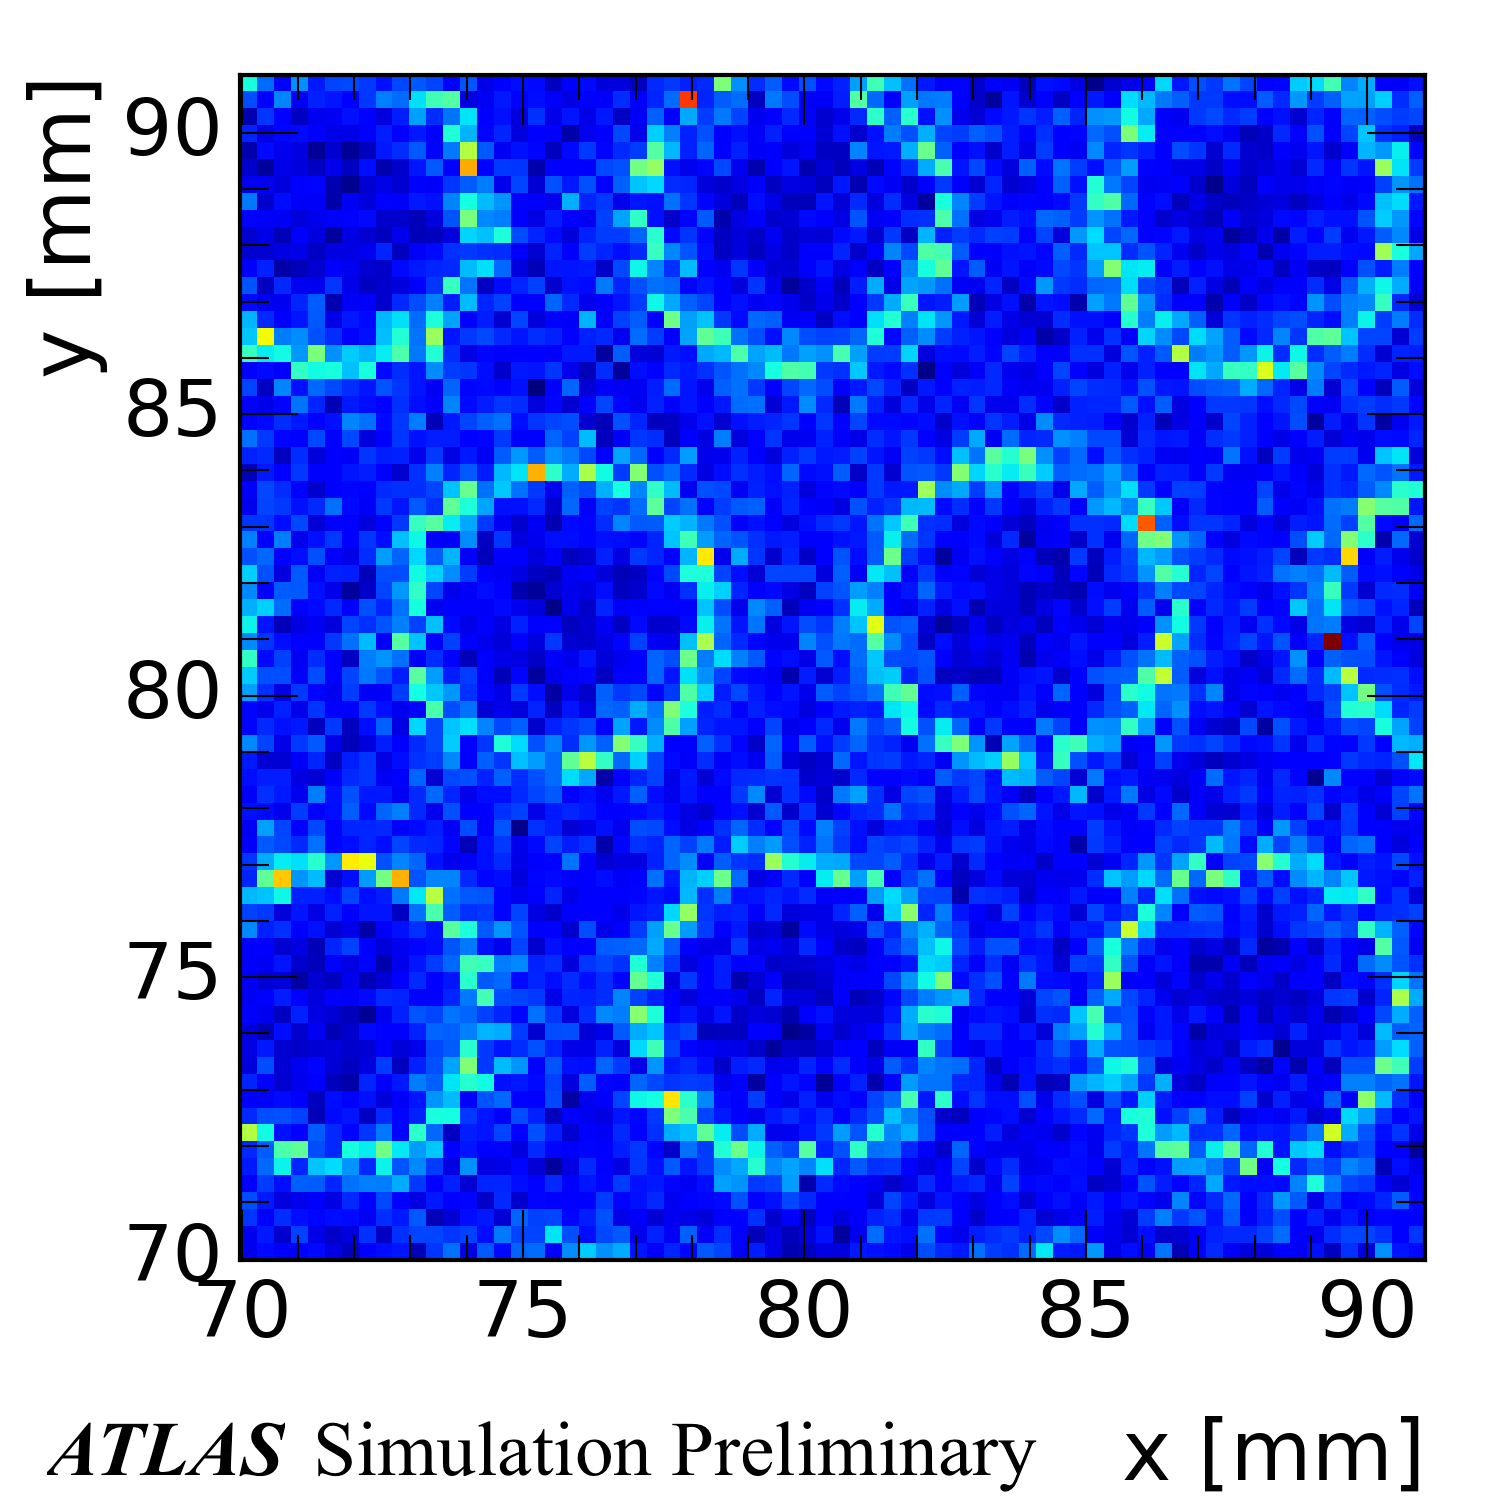
\includegraphics[width=0.5\linewidth]{MC/xySumE.png} }
%\caption{Shower energy response histogram in the x vs y plane for electrons, generated with uniformly distributed x and y and energy less than 1 GeV. Light circles are corresponding to a showers, started inside a LAr gaps with on average higher energy response, while the dark parts are corresponding to dead material respectively with smaller sum of the "hits" energy. }
%\label{fig:FSFluctuations}
%\end{figure}




\begin{figure}[!b]
\begin{minipage}[h]{0.49\linewidth}
\center{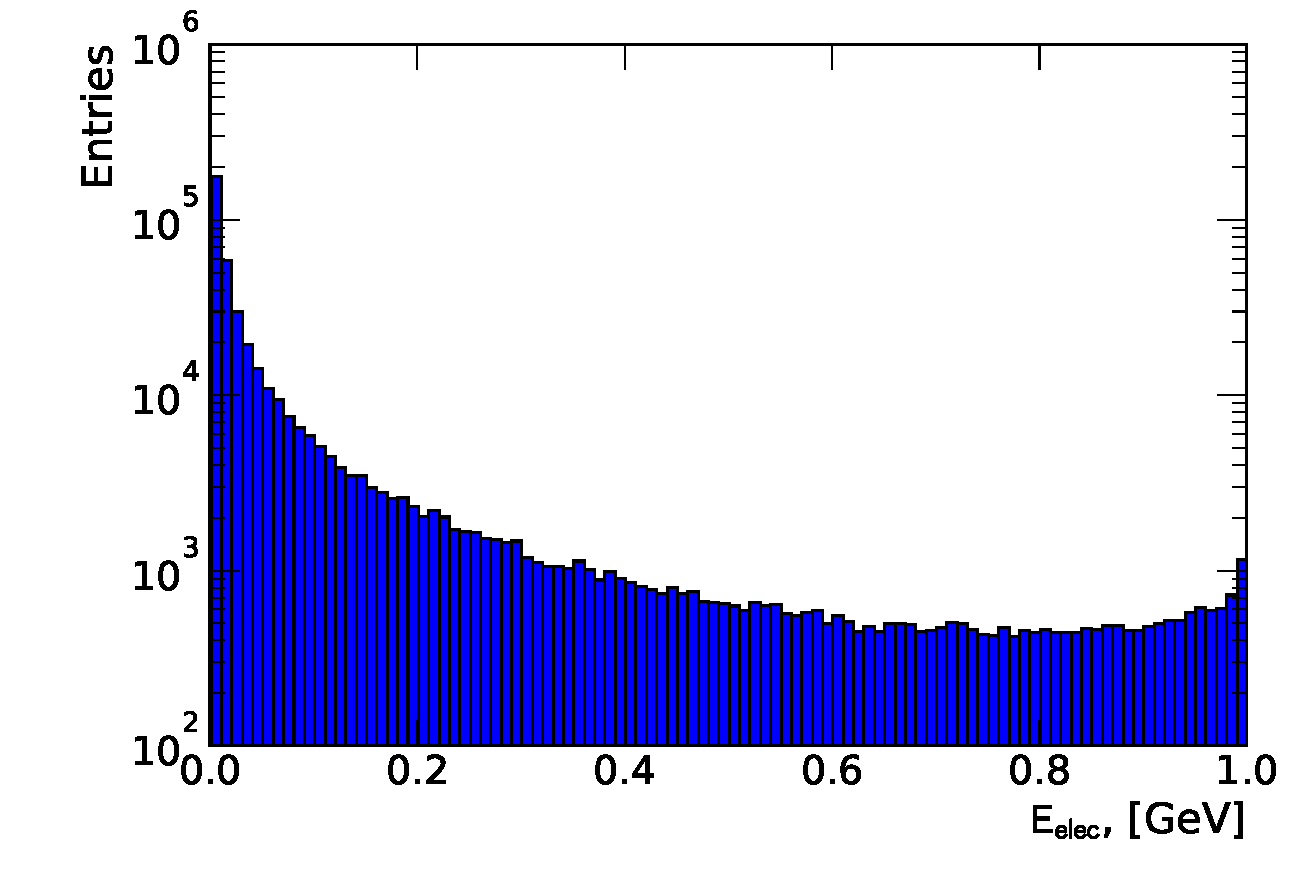
\includegraphics[width=1.0\linewidth]{MC/FSEnergy.pdf}  \\ a)}
\end{minipage}
\hfill
\begin{minipage}[h]{0.49\linewidth}
\center{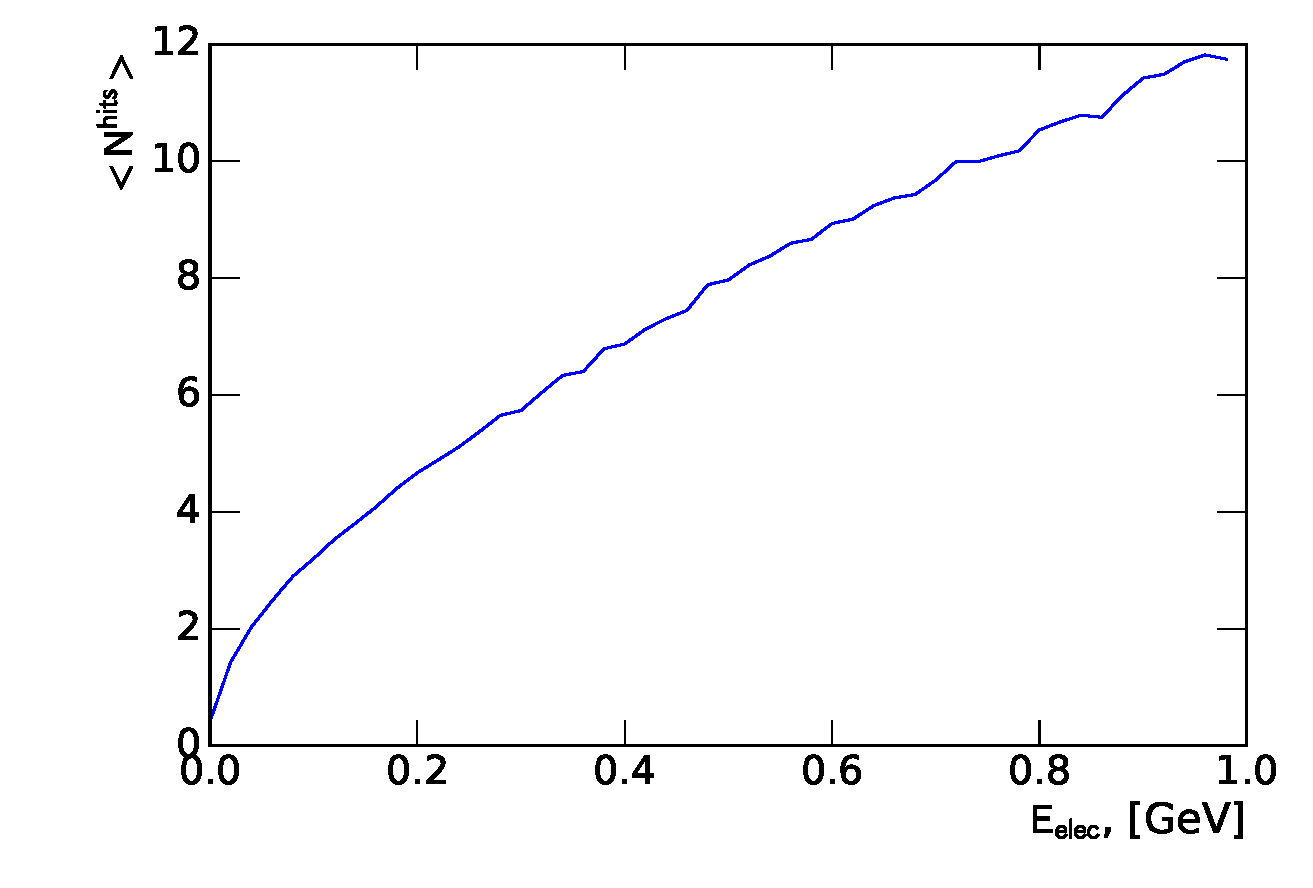
\includegraphics[width=1.0\linewidth]{MC/nHitsMean.pdf} \\ b)}
\end{minipage}
\caption{Distribution a) electron energies and b) mean number of hits in a shower vs energy of electron for electrons with energy less than 1 GeV coming from initial electron with energy 1 TeV. }
\label{fig:TrackEnergy}
\end{figure}

Fast simulation of forward calorimeters (FCAL) is a complicated task due to its complex structure. As it was mentioned in a Sec. ~\ref{sec:forwardCalo} FCAL consists of hexagonal absorber cells with anode tube and cathod rod in the cell center and liquid argon in the gap between rod and tube. In order to simulate resolution of high energetic electrons, good fast simulation technique should take this feature of large amount of non-uniformly distributed sensitive material.

Resolution of electron inside calorimeter can be written as:
\begin{equation}\label{eq:EMResoultion}
\frac{\sigma}{E} \approx \frac{1}{\sqrt{E}}	\oplus \frac{1}{E} 	\oplus const,
\end{equation}
where symbol $\oplus$ indicates a quadratic sum. The first term is 'stocastic term', which includes intrinsic shower fluctuations, second takes into account readout noise effects and pile-up fluctuations. Constant term derives from non-uniformities in a detector, causing large fluctuation of the energy loss. Resolution of high-energy electrons is mostly dominated by the constant term. 

Fluctuations due to a detector design are visible in a simulation of small energy electrons, generated inside a different points in forward calorimeter. Shower energy $E^{shower}$ distribution in the x vs y plane is showed on Fig. \ref{fig:FSFluctuations}, where shower energy is defined as:
\begin{equation}
E^{shower}=\sum E_i^{hits},
\end{equation}
where $E_i^{hits}$ is an energy of i-th shower deposit inside sensitive material. Periodic structure resembles the calorimeter design, where light circles are corresponding to gaps with liquid argon. It could be reduced to a 1-d problem by introducing $d_{rod}$ distance to a closest rod center. 

Typical electron substituted by a frozen showers coming from a simulation of high energy electrons have a relativelly small energy (Fig. ~\ref{fig:TrackEnergy} a)). Mean number of depositions in a sensitive material in a "frozen" shower is around 5 and this value rises with electron energy (Fig. ~\ref{fig:TrackEnergy} b).  Fig. ~\ref{fig:FSProduction} presents a distribution showers for electrons with energy below 1 GeV coming from initial electrons with energy 1 TeV in the distance to a closest rod center vs shower energy plane. Liquid argon gap is marked by a red lines. There is a clear difference in a showers energies between electrons born in a sensitive and dead material. Difference in a shower properties are also visible for number of hits  (Fig. ~\ref{fig:ShowerProp} a) and standard deviation energy of hits in shower (Fig. ~\ref{fig:ShowerProp} b) distributions. Size of this differences depends on a electron energies and higher for a smaller energies (Fig. ~\ref{fig:FSProduction2} a) and less significant for a higher energies (Fig. ~\ref{fig:FSProduction2} b).  This fact combined with energy distribution states an importance of proper simulation non-uniformities for showers coming from a small energy electrons.





\begin{figure}[!tbp]
\center{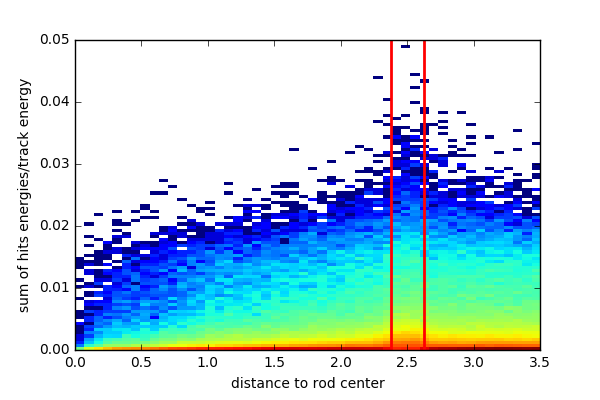
\includegraphics[width=1.\linewidth]{MC/fullBinningScatter.png} }
\caption{Distribution of electron showers for electrons with energy less than 1 GeV coming from initial electron with energy 1 TeV in distance to a closest rod center vs shower energy plane. Position of a liquid argon gap is noted by a red lines. There is visible difference in shower properties between showers inside and outside of the liquid argon gaps}
\label{fig:FSProduction}
\end{figure}

\begin{figure}[!tbp]
\begin{minipage}[h]{0.49\linewidth}
\center{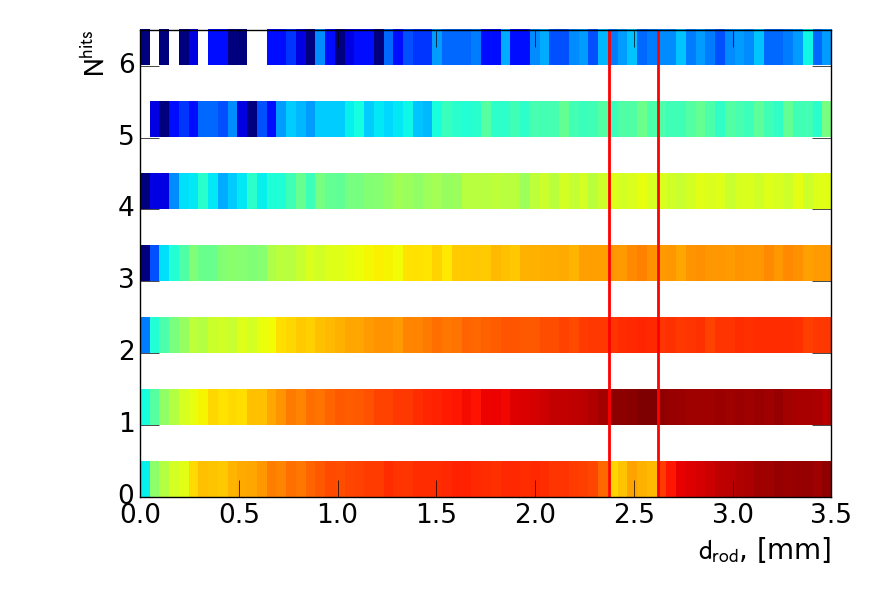
\includegraphics[width=1.0\linewidth]{MC/nHits.png}  \\ a)}
\end{minipage}
\hfill
\begin{minipage}[h]{0.49\linewidth}
\center{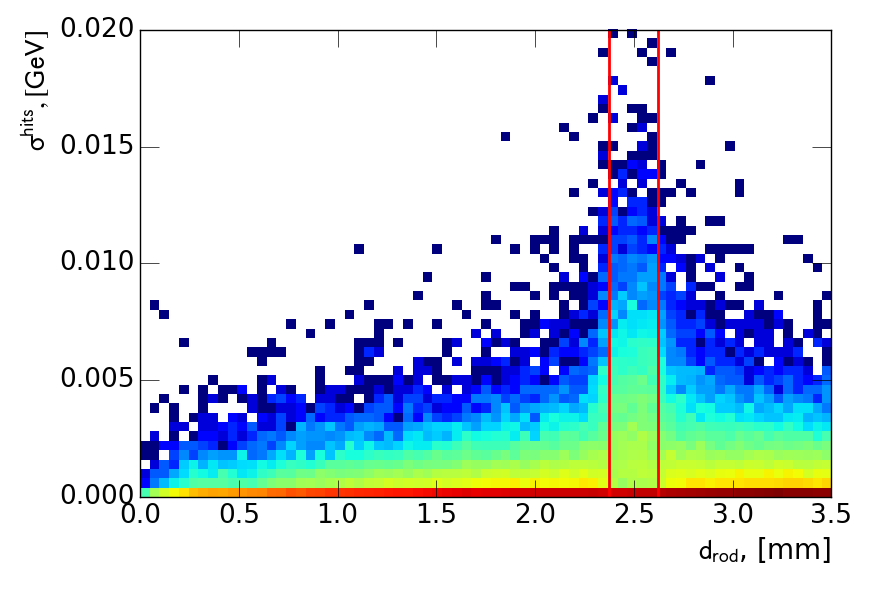
\includegraphics[width=1.0\linewidth]{MC/rms.png} \\ b)}
\end{minipage}
\caption{Distribution of electron showers for electrons with energy less than 1 GeV coming from initial electron with energy 1 TeV in distance to a closest rod center vs a) number of hits in a shower plane and b) standard deviation of hits in a shower energy. Position of a liquid argon gap is noted by a red lines. There is visible difference in shower properties between showers inside and outside of the liquid argon gaps}
\label{fig:ShowerProp}
\end{figure}

\begin{figure}[!tbp]
\begin{minipage}[h]{0.49\linewidth}
\center{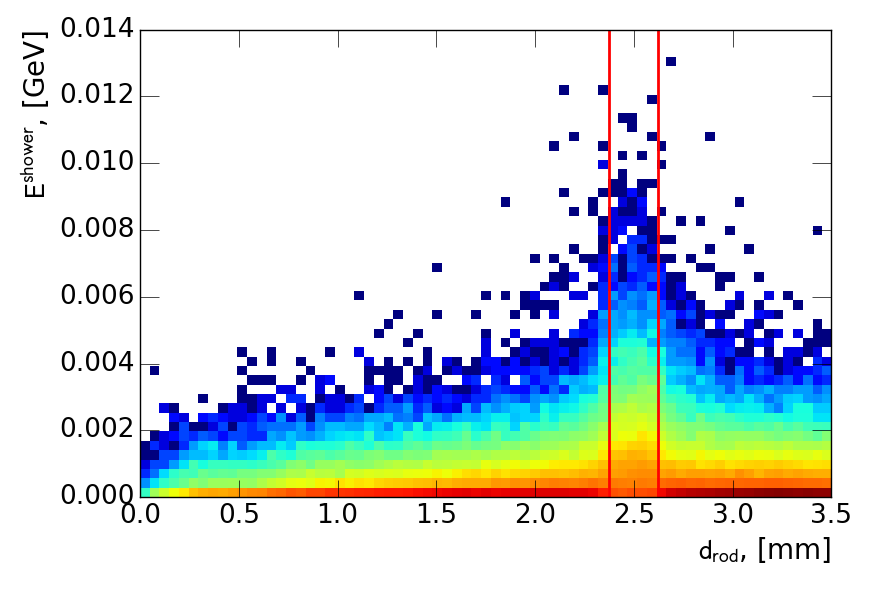
\includegraphics[width=1.\linewidth]{MC/fullBinningScatterSmall.png} \\ a)}
\end{minipage}
\hfill
\begin{minipage}[h]{0.49\linewidth}
\center{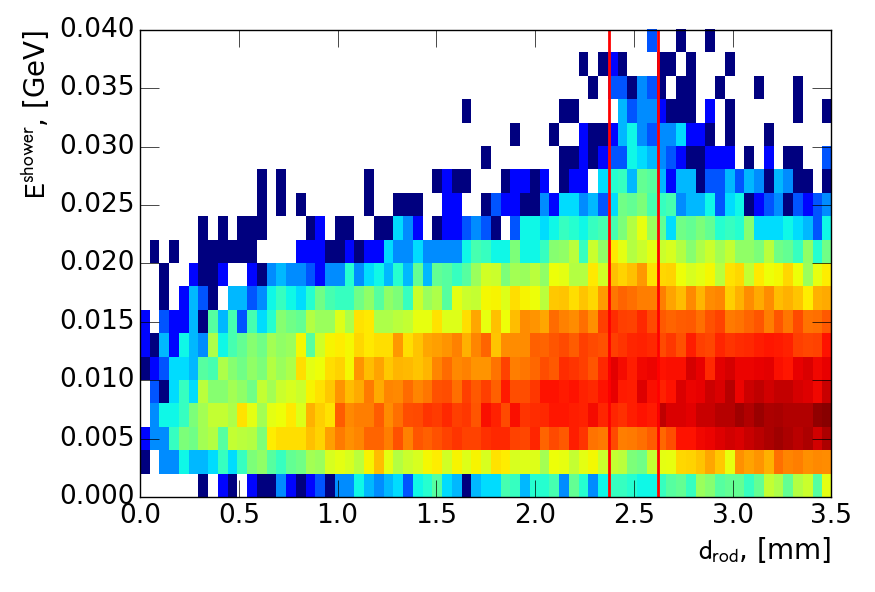
\includegraphics[width=1.\linewidth]{MC/fullBinningScatterBig.png} \\ b)}
\end{minipage}
\caption{Distribution of electron showers for electrons with energy a) less than 100 MeV  and b) higher than 300 GeV coming from initial electron with energy 1 TeV in distance to a closest rod center vs shower energy plane. Position of a liquid argon gap is noted by a red lines. Size of the difference in a shower properties depends on the energy of the electrons and higher for smaller energies}
\label{fig:FSProduction2}
\end{figure}

On another hand, use of the frozen showers in a small energy region can be suboptimal because of the small number of energy depositions in a shower. For electrons with energy less than 30 MeV 90\% of the showers has zero depositions and just 0.5\% of showers are having more than 1 hits (Fig. ~\ref{fig:fracHits}). Below this energy single energy spot model have showed better performance in simulation.

\begin{figure}[!tbp]
\begin{minipage}[h]{0.49\linewidth}
\center{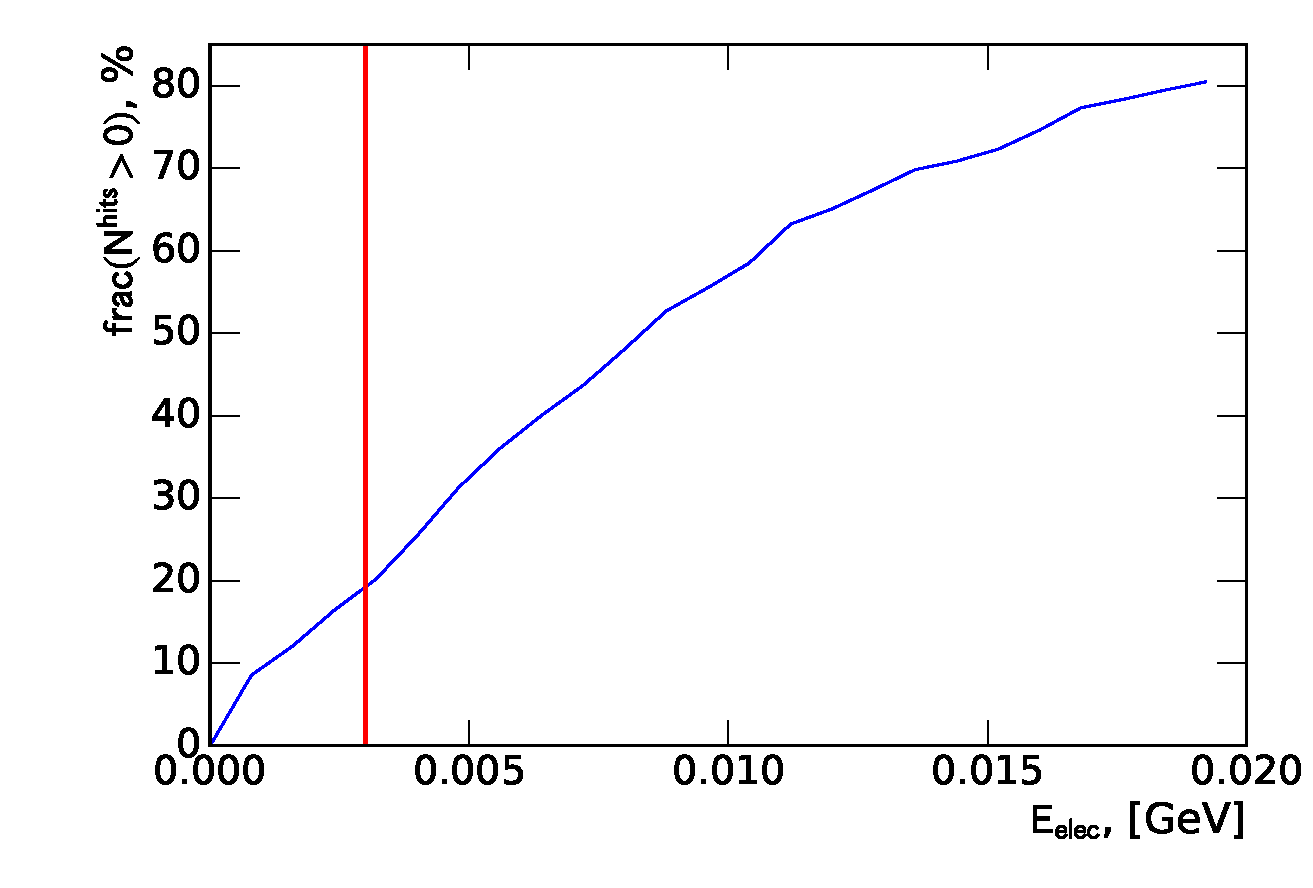
\includegraphics[width=1.\linewidth]{MC/fracHits2.pdf} \\ a)}
\end{minipage}
\hfill
\begin{minipage}[h]{0.49\linewidth}
\center{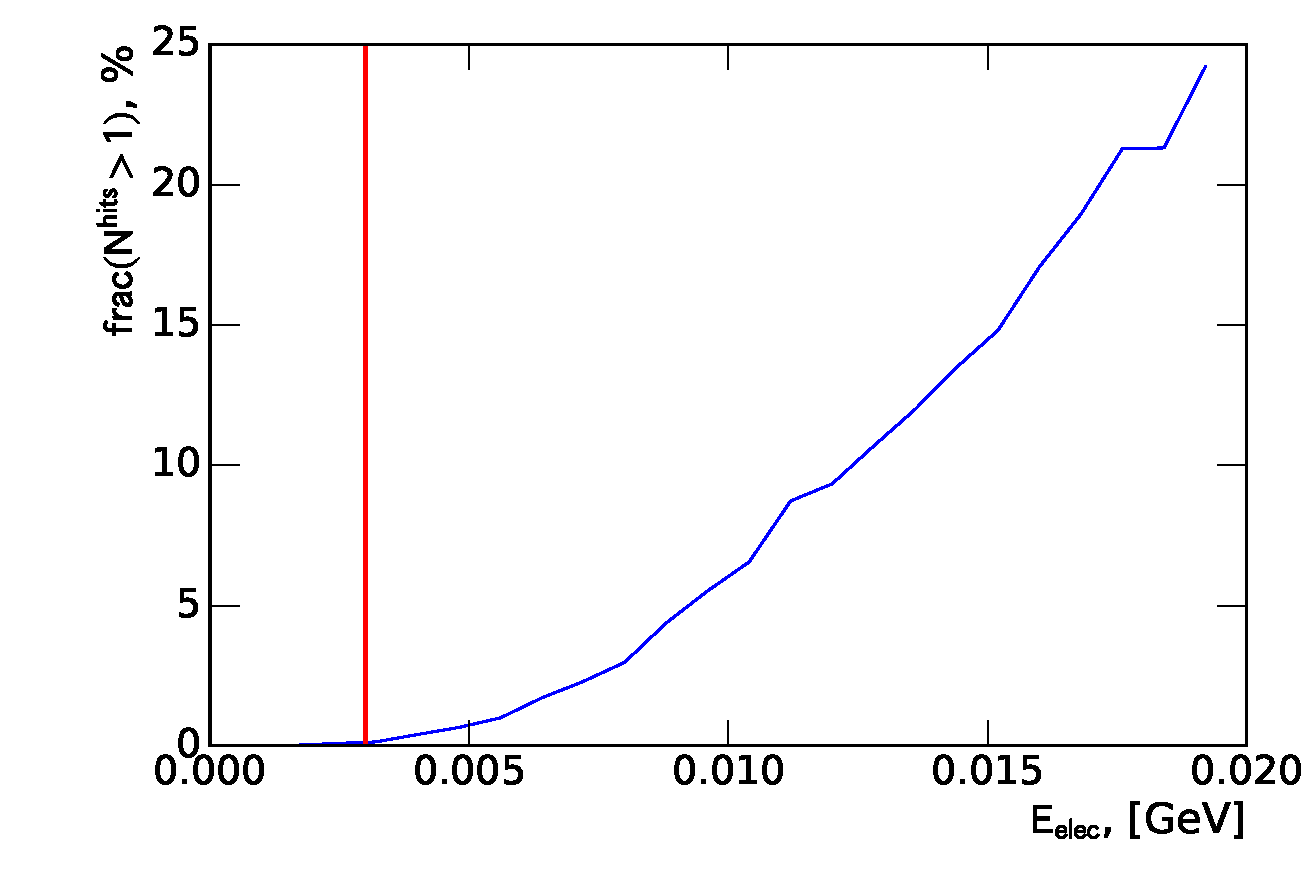
\includegraphics[width=1.\linewidth]{MC/fracHits.pdf} \\ b)}
\end{minipage}
\caption{Distribution of fraction of showers with a)at least 1 b) at least 2 depositions inside sensitive material depending on a initial electron energy. Red line denotes 30 MeV lower limit for a frozen showers method.}
\label{fig:fracHits}
\end{figure}


\section{Generation and use in simulation}

As it was mentioned in introduction frozen showers method consist of the 2 stages: generation of libraries and use in simulation. Generation needs to be repeated for each significant change in a physics processes description in Geant4 or in a description of detector. Showers are stored in a library in pseudorapidity and distance to a closest rod center bins, while energy remains unbinned. Distance binning was introduced to describe fluctuations from Sec. \ref{sec:FSproblem}. Position of the liquid argon gap bin is corresponding to a real gap position. 

In order to have proper energy distribution for a generation of library particles coming from a simulation of physical process (usually $t\bar{t}$ or high energy electrons) are used. For each particle eligible for frozen showers use parameters are saved in a HepMC (reference) format for a later use. On a second stage, these particles are propagated through the calorimeter using standard \atlas simulation infrastructure. Each hit is saved as a shower inside library in a corresponding pseudorapidity and distance bin. 

Additionally, in order to save disc space as well as a memory consumption, hit information is compressed. This compression is done in a two steps: 
\begin{description}
\item [Hit merging] if the distance between any two hits is smaller, than a given parameter $R_{min}$, then hits are merged into one deposit at the energy weighted center of them. This process is done iterativelly.
\item [Truncation] hits whose energies are below the fraction f of the total energy sum of all hits, are truncated. The energy of remaining hits is rescaled back to preserve the total deposited energy.
\end{description}

During simulation, if an energy of a particle falls below cut-off energy, the particle algorithm examines resulting shower containment. It checks  that particle is far from the edges of calorimeter, so what shower will be by 90\% inside calorimeter. This depends also on a energy of particle, because shower sizes are growing with energy. The algorithm searches for a shower with the closes energy in a corresponding pseudorapidity and distance bin. Shower is a rotated in a direction of particle. In order to correct differences in energy, each hit in a shower is scaled as:
\begin{equation}
E_{hit}^{new}=E_{hit}\cdot \frac{E_{part}}{E_{part,lib}},
\end{equation}
where $E_{hit}$ is the energy of the hit, $E_{part}$ is the energy of the particle and $E_{part,lib}$ is the energy of the particle from a library. Then particle is removed and substituted by a resulting shower. Later, reconstruction algorithm uses hits from a frozen shower as a usuall energy depositions in a sensitive material. 

\begin{figure}[!tbp]
\center{
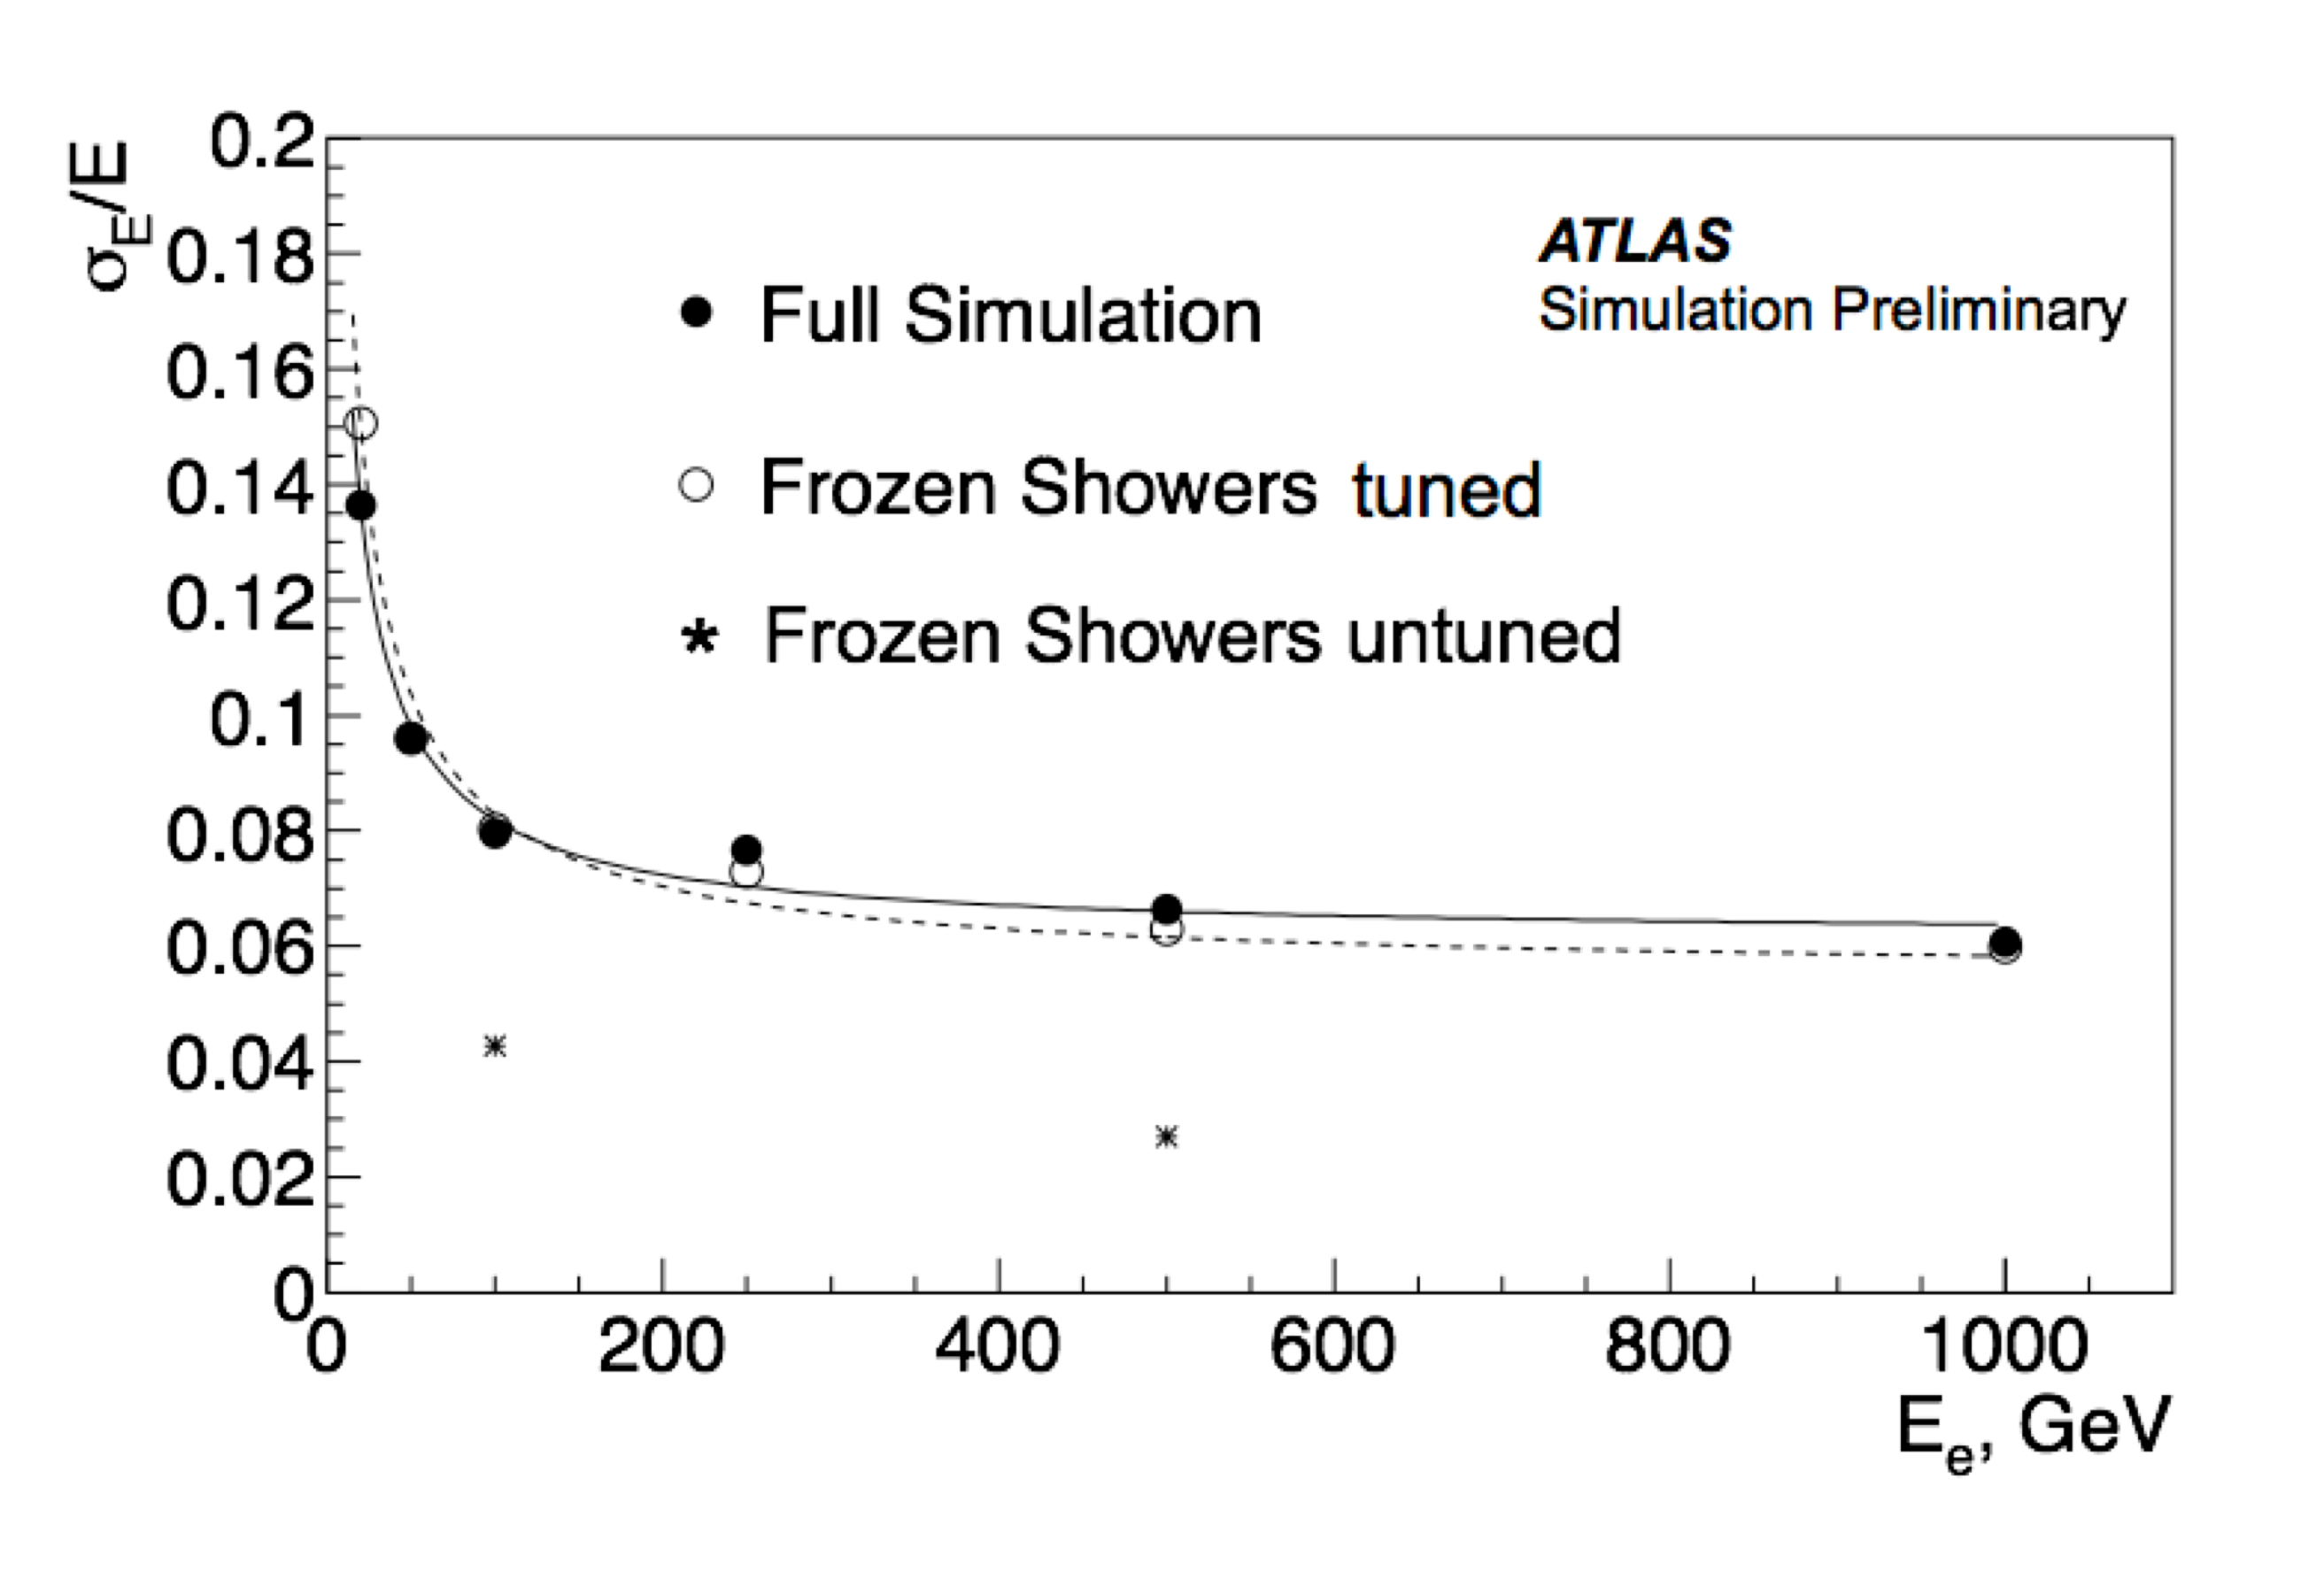
\includegraphics[width=0.8\textwidth]{MC/fs.png}
\caption{Electron resolution for full simulation, tuned and untuned frozen showers. Electrons simulated with frozen showers libraries before tuning (star points) have twice smaller resolution, than an electrons from full simulation (circles). Tuning (black dots) is allowing to gain better agreement with full simulation.}
\label{fig:FS_resolution}}
\end{figure}

\begin{figure}[!tbp]
\center{
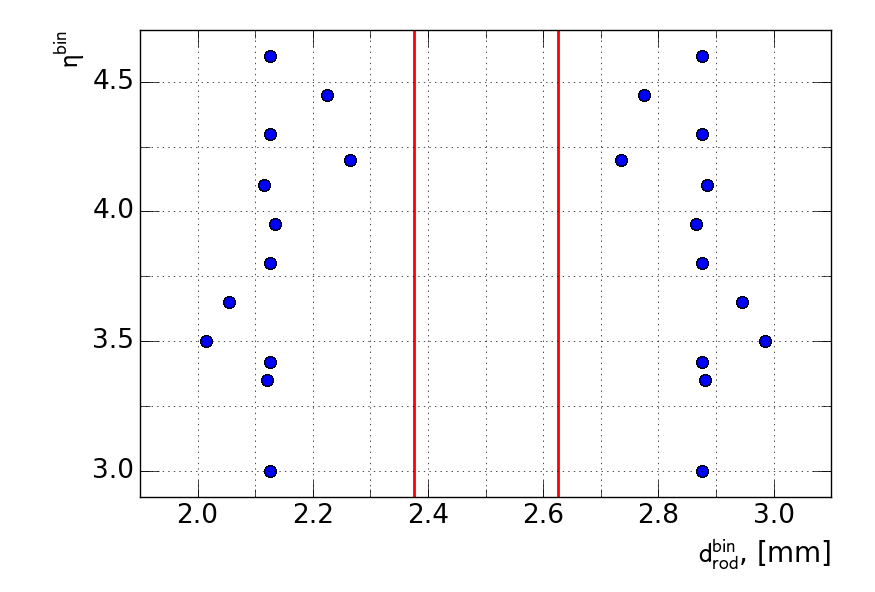
\includegraphics[width=0.8\textwidth]{MC/oldTuning.png}
\caption{Position of gap bins for different $\eta$ bins in old libraries after tuning. Dots are corresponding to a limits of each bin. Red lines are denoting original position of bins, that are corresponding to a position of a liquid argon gap in the calorimeter.}
\label{fig:FSOldTuning}}
\end{figure}

\subsection{Libraries tuning}

Frozen showers method gives a good agreement with a full simulation for a shower shape variables(Sec. \ref{sec:FSValidation}), however resolution of the reconstructed electrons is around 2 times smaller(Fig. ~\ref{fig:FS_resolution}), than in a full simulation. It can be interpreted as a lack of the showers from liquid argon gap in a simulation. Most of this effect is coming from an electron libraries. This means that this libraries are requiring additional reconstruction-based tuning after generation.

Usual tuning consists of 2-step manual procedure:
\begin{description}
\item [Changing bin width] On this stage width of the liquid argon bin is enlarged. This is causing larger size of the fluctuations, that leads to a higher resolution and a mean energy of reconstucted electrons
\item [Shower energy scaling] In order to correct introduced shift in a mean energy shower energy is reduced by rescaling all of the hits in a shower.
\end{description}
 It is repeated iterativelly in each pseudorapidity bin separately till the desired agreement is obtained. The resulting bin positions are shown on a Fig.  ~\ref{fig:FSOldTuning}. This method allows to have a relatively good agreement with full simulation (black dots on Fig. ~\ref{fig:FS_resolution}). However, it is necessary to repeat this procedure for each new libraries generation and requires significant tuning effort, that makes it not optimal. 

\section{Machine learning based bin finding procedure}

Since frozen showers are planned to be used in Run-2 Monte-Carlo production, there is a need for a more automatic procedure of library generation with proper electrons resolution. One of the possible ways is to choose different position of liquid argon bin during libraries generation using machine learning tools. In this section automatic bin finding procedure will be discussed.
\subsection{Machine learning introduction} 

Machine learning is a set of algorithms, what allows computers to learn and give a predictions without being specifically programmed. This is a modern field of computer science, that is wildly used in a different fields like computer vision, natural language processing, data science etc. There are two main types of machine learning algorithms: supervised, where example of desired output is given by the "teacher" and the goal is to learn a general rule, that maps inputs to outputs and unsupervised learning, then there are no labels given to algorithm, and algorithms is discovering hidden patterns in data. Initial data parameters of interest, that are used in algorithm to learn are called features. 

Machine learning algorithms can be used for solving a classification problem, where each event should be identified to one of the specified classes. Since the first introduction of the machine learning classifiyng algorithms called perceptron by a Rosenblatt <ref> many different algorithms have been invented. In this analysis decision trees and support vector machines have been used.

\subsubsection{Binary decision trees}

Binary decision trees are one of the most commonly used machine learning algorithms for a classification problems in a particle physics. Schematic representation of this algorithm is shown on a Fig. ~\ref{fig:MLAlgo} a. Each node is corresponding to the one of the internal input variables and connected to two branches, that are split in the respect to the a variable. The first node is called a root node. Depth of the tree is a number of edges from the node to the tree's root node. Leaf node represents classification or decision.
 For each node the best feature is selected and it's cut value are obtained by calculating each possible variation in the feature set and then ranking them. One of the main advantages of the decision trees is a simplicity of visualization and interpretation. 

\subsubsection{Support vector machines}

\begin{figure}[!tbp]
\begin{minipage}[h]{0.49\linewidth}
\center{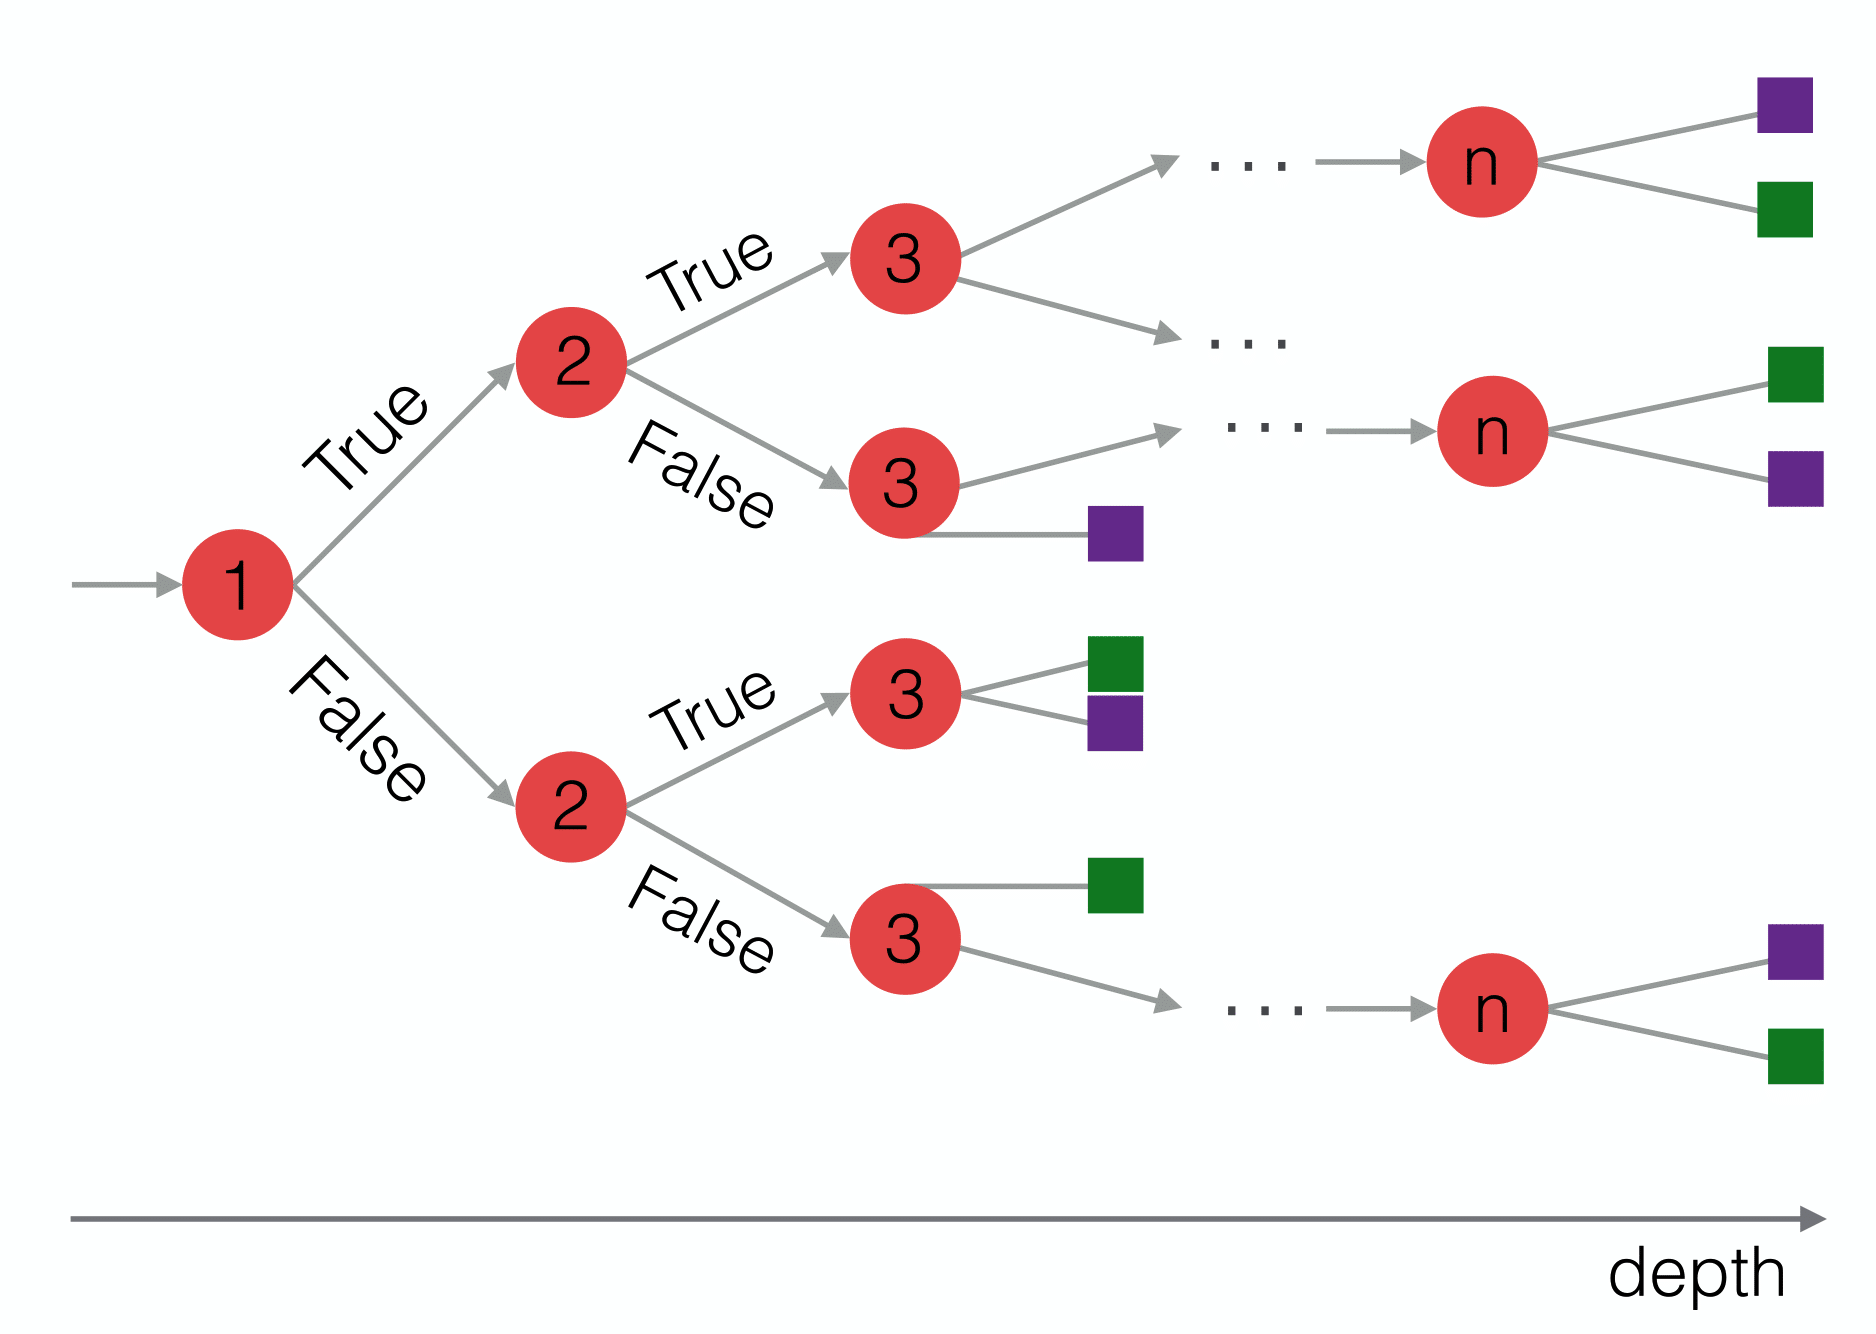
\includegraphics[width=1.\linewidth]{MC/DecisionTree.png} \\ a)}
\end{minipage}
\hfill
\begin{minipage}[h]{0.49\linewidth}
\center{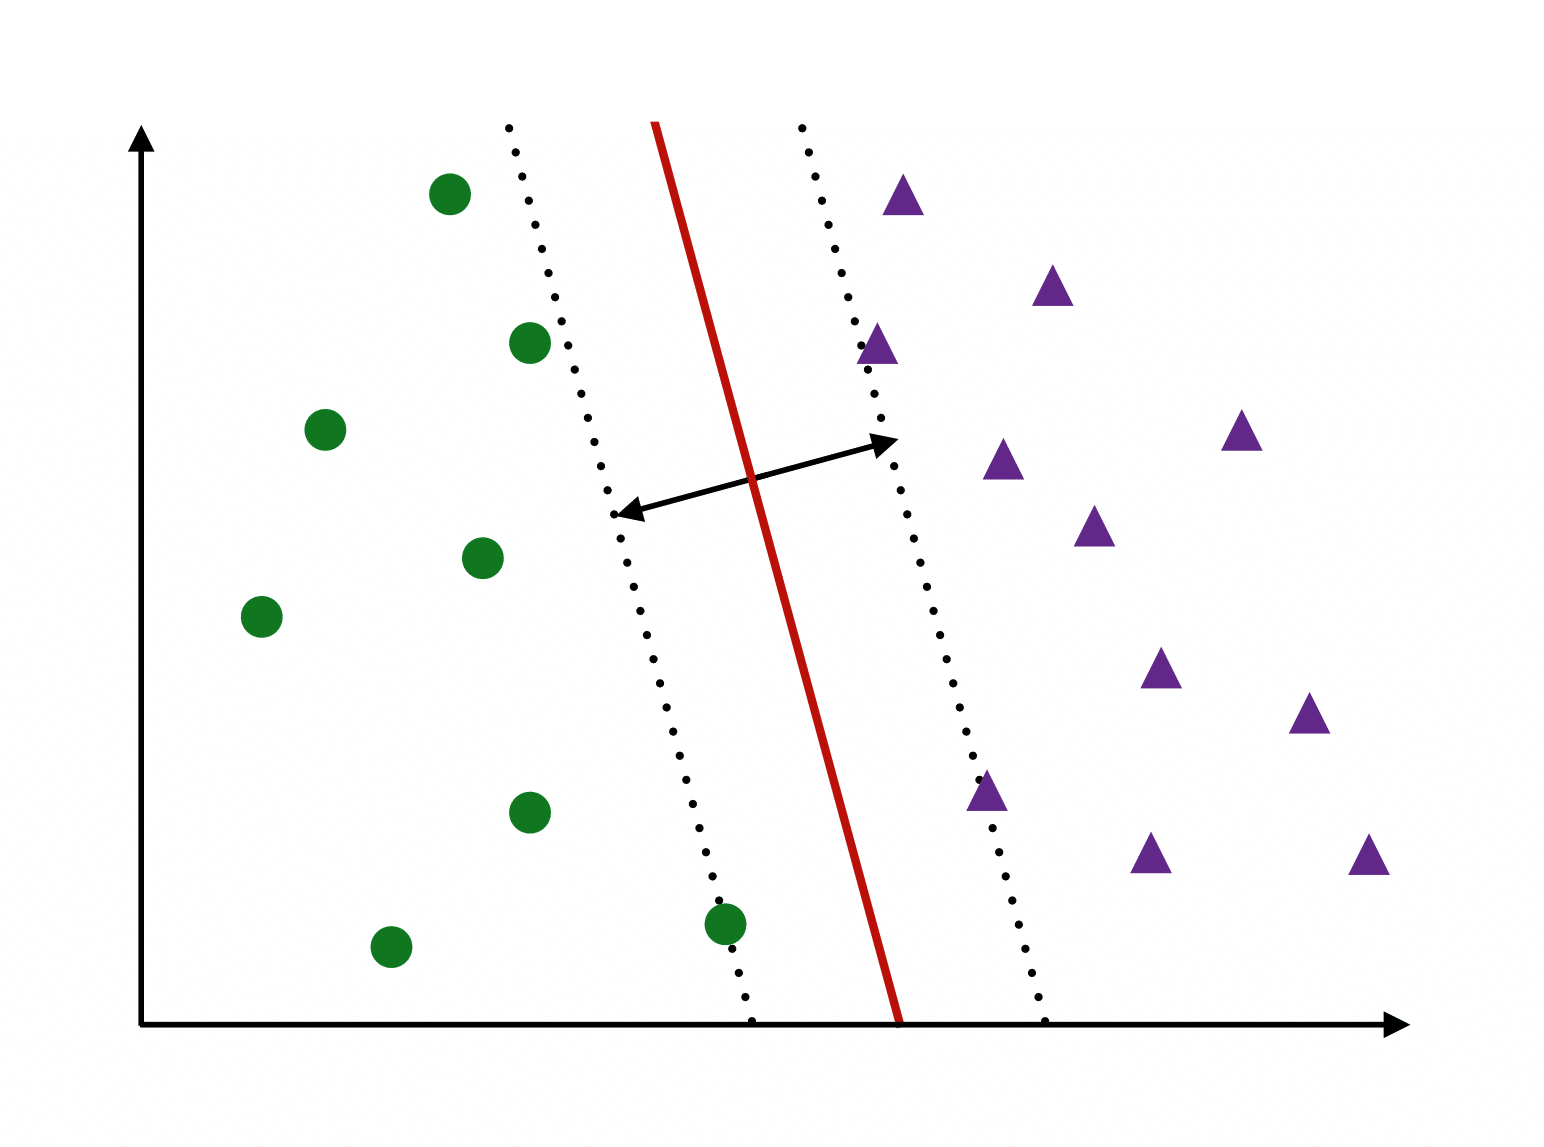
\includegraphics[width=1.\linewidth]{MC/SVM.png} \\ b)}
\end{minipage}
\caption{Schematic representation of machine learning algorithms, used in the analysis for a classification. Green figures are representing first class of the events, whereas violet ones belong to a second class.  
a) Representation of a binary decision tree structure: red circles are corresponding to a node, that are split in the respect to the one of the features. Squares represent leafs, where all of the events are classified to a certain class. Depth of the tree is calculated as a number of edges from the node to the trees first node. 
b) Representation of the SVM algorithm. Dividing hyperplane is shown by a solid line. The dashed lines represent the maximum margin boundaries}
\label{fig:MLAlgo}
\end{figure}

Support vector machines (SVM) is a supervised machine learning algorithm which can be used for classification problems. In this algorithm each event is represented in a p-dimensional parameter space. Classification is performed by finding a the hyper-plane that differentiate the two classes with the largest separation (Fig. ~\ref{fig:MLAlgo} b). The hyperplane can be written as the set of points $\vec {x}$ in a parameter space satisfying:
\begin{equation}
\vec{w}\cdot \vec{x} - b = 0,
\end{equation}
where $\vec{w}$ is the normal vector to the hyperplane and the parameter $\frac {b}{\|{\vec {w}}\|}$ determines the offset of the hyperplane from the origin along the normal vector $\vec {w}$. The margin hyperplanes are described by equations:
\begin{eqnarray}
\vec{w}\cdot \vec{x} - b = 1, \\
\vec{w}\cdot \vec{x} - b = -1,
\end{eqnarray}
where $\frac{2}{\|\vec{w}\|}$ is the distance between these 2 hyperplanes, so planes with the maximum margin between should have the minimum $\|\vec{w}\|$. 

Because we want to prevent each point to fall into the margin, we following constrain should be satisfied: 
\begin{eqnarray}
\vec{w}\cdot \vec{x} - b \geqslant 1 \textrm{ where } y_i = 1,\\
\vec{w}\cdot \vec{x} - b \leqslant -1 \textrm{ where } y_i = -1,
\end{eqnarray}
These equations can be rewritten as:
\begin{equation}
y_i(\vec{w}\cdot \vec{x} - b ) \geqslant 1
\end{equation}

It is also possible to construct a non-linear classifier by replacing dot-product with a differen \textit{kernel} function. In this thesis, a radial basis function (RBF) kernel is used:
\begin{equation}\label{eq:RBF}
K_{rbf}(\vec{x}_i, \vec{x}_j) = e^{-\gamma | \vec{x}_i - \vec{x}_j|^2} \, \gamma >0,
\end{equation}
where parameter $\gamma$ adjusts the width of the kernel.


\begin{figure}[!t]
\center{
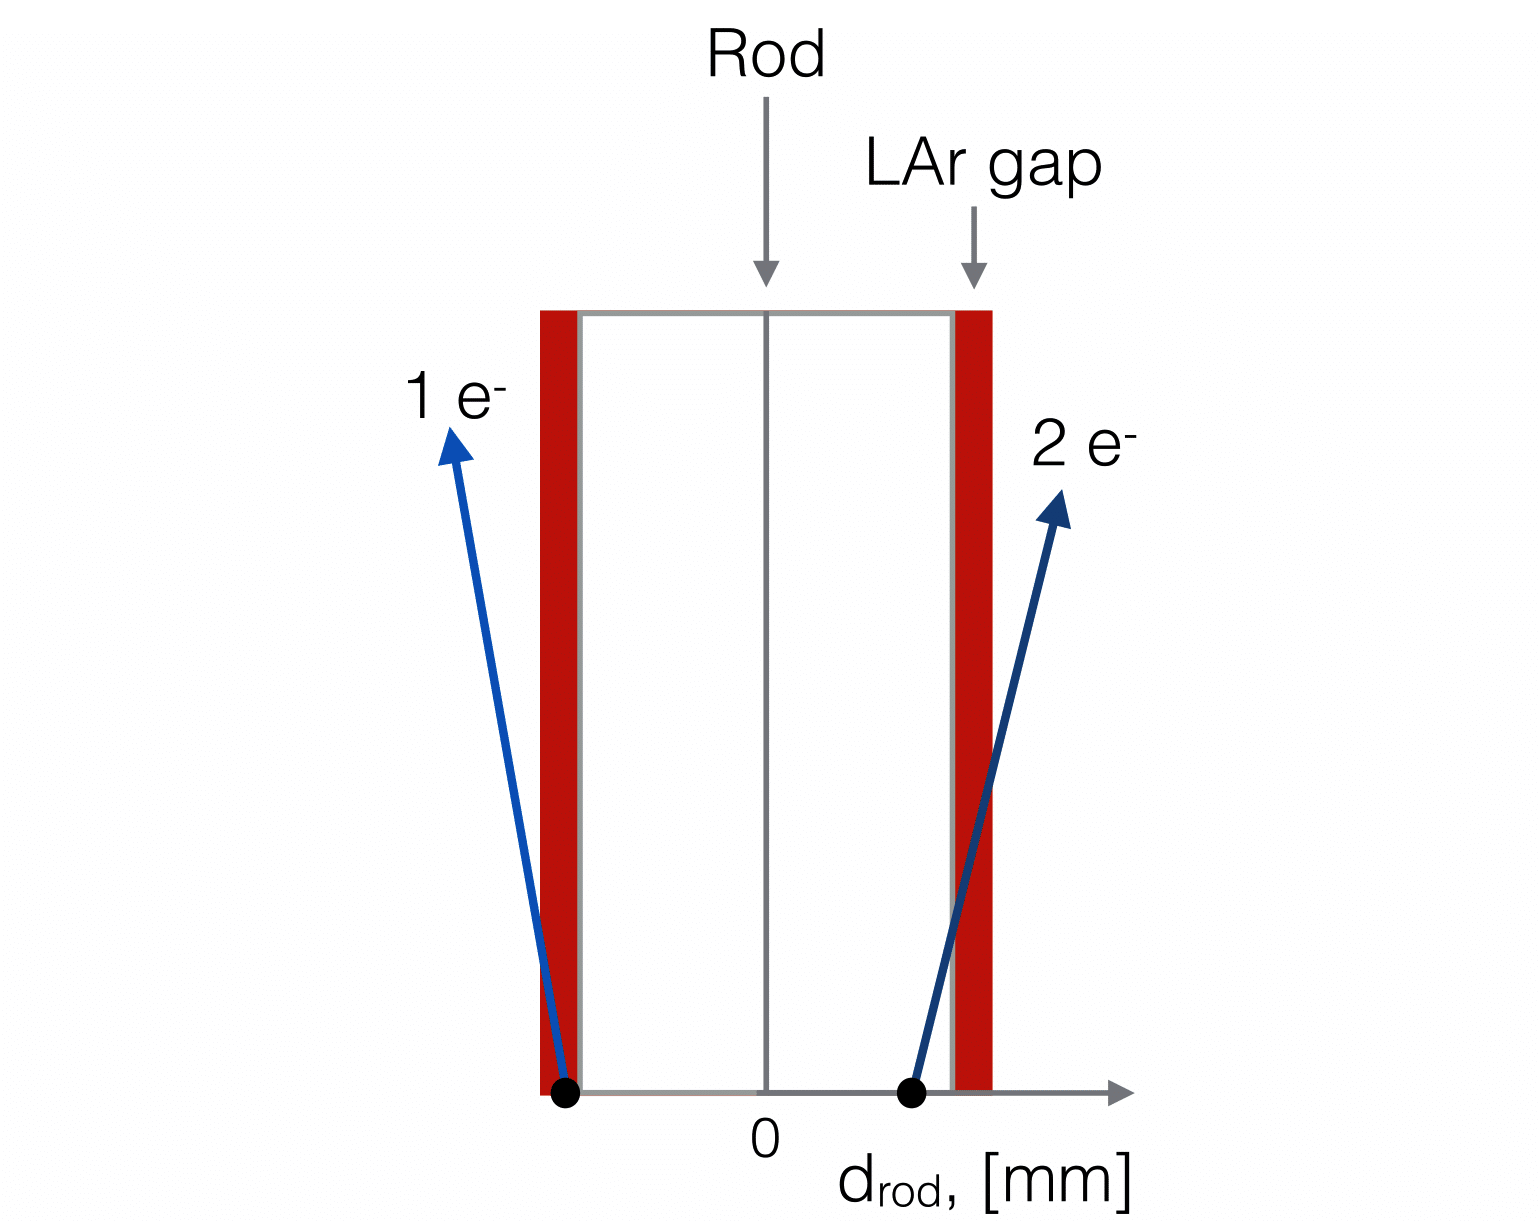
\includegraphics[width=0.5\textwidth]{MC/Model2.png}
\caption{Schematic representation of the model. Electron 1 is created in a liquid argon gap. Electron 2 is created near liquid argon gap and crosses it. This causing a smearing of sensitive material showers distribution. Electrons created in a sensitive material tend to create more energetic showers, than electrons from a dead material. However, electrons, shown on this scheme, may give similar shower and therefore be not distinguishable.}
\label{fig:Model}}
\end{figure}

\subsection{Model description}



As it was mentioned in a previous sections, modules in FCAL are consisting of different types of material and showers started inside dead material are usually having smaller energies, than a sensitive material once. However, the validation (Fig. \ref{fig:FS_resolution}) can be interpreted as the that there are high energy showers outside of the liquid argon gap. It could be explained by the fact, that electron, created in a dead material, can cross a liquid argon gap and give a hit there as it shown in Fig. \ref{fig:Model} (electron 2). These electrons would be indistinguishable from electrons, created directly in a sensitive material (electron 1 in Fig. \ref{fig:Model}). 

It was decided to treat this electrons together with electrons created in sensitive material, and call a caused showers as a sensitive material showers. Oppositely, showers that did not crossed a liquid argon gap, are called a dead material showers. This model leads to a bigger gap.  

From the definition, this model leads to the dependency of the liquid gap width on:
\begin{description}

\item [Electron energy] Gap should get wider with higher energy of the initial electron, because of the growth of the mean free path with energy.
\item [Direction of the electron] Electron aligned collinearly with liquid argon gap will have smaller probability to cross liquid argon gap. This probability will grow with the angle reaching its maximum at  $90^{\circ}$

\end{description}

\subsubsection{Training sample}

Real distributions, used in simulation, have a complicated structure and depend on a physical processes simulated. Machine learning could catch these dependencies, instead of the needed ones. This is why a more simplified data as a training sample for machine learning  is needed.  Training sample was made by a simulation of the electrons, created in forward calorimeters. In order to treat equally high and low initial electron energy showers, the uniform distribution of the energies is used.

Most of the showers have direction in $\eta$ range between 3.0 and 5.0 (Fig. \ref{fig:EtaMomVsEnergy}), that is corresponding to a position of the calorimeter. Distribution of the showers directions in different positional $\eta$ bins shows, that there is indeed the correlation between direction and the position of the electrons. Because of this it was decided to use an electrons with direction, uniformly distributed between 3.0 and and 5.0.


\begin{figure}[!tbp]
\center{
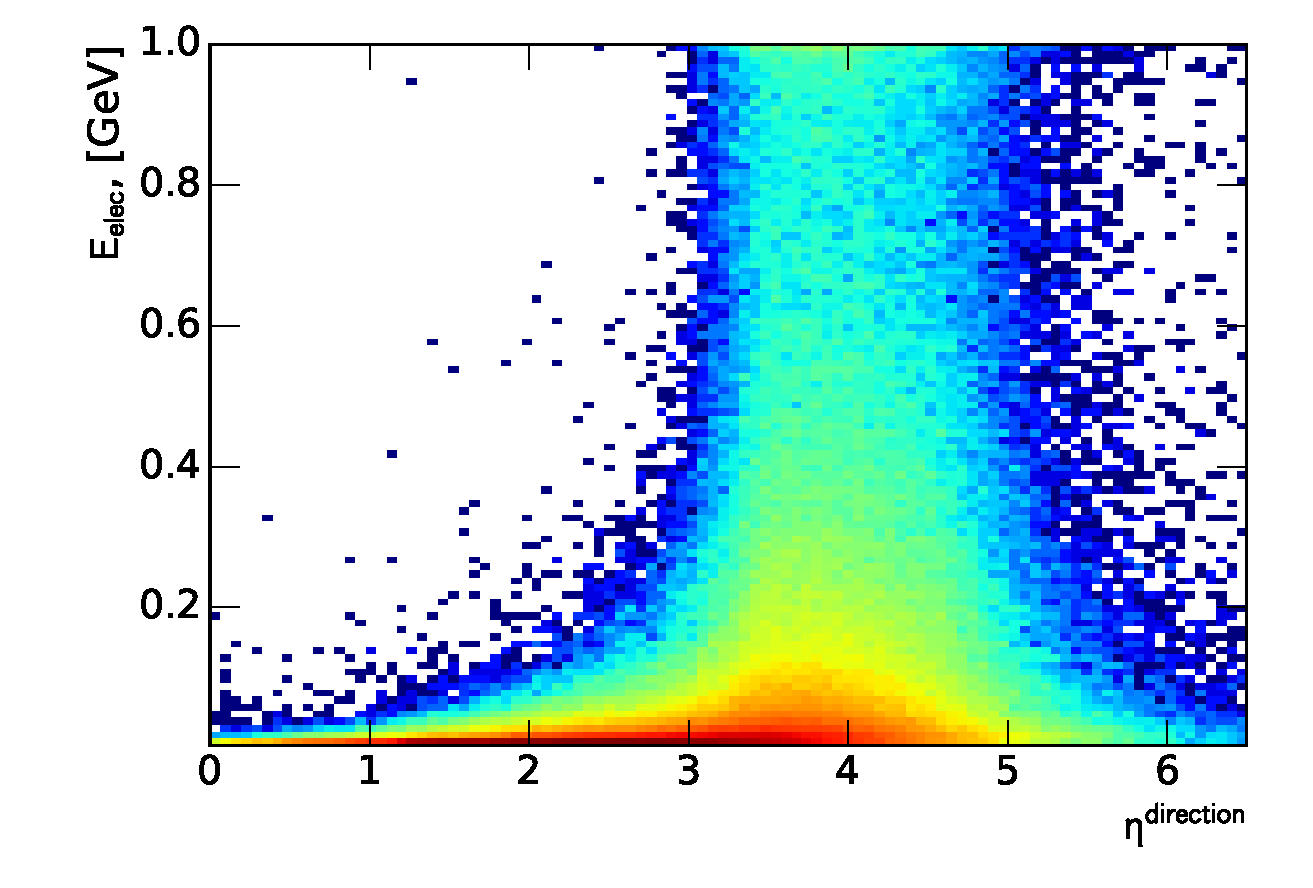
\includegraphics[width=0.8\textwidth]{MC/FSEtaMomVsEnergy.pdf}
\caption{Distribution of showers used in production of 1000 GeV electrons on shower energy vs $\eta_{momentum}$ plane.}
\label{fig:EtaMomVsEnergy}}
\end{figure}

\subsubsection{First classifier}

First classifier classifier aims to classify all of the showers based on a shower parameters. It is possible to train supervised learning algorithm on pre-labeled artificially reduced training sample and then expand the classification on a full train sample. 

Pre-labeling could be easily done from a definitions of sensitive and dead material showers based on a distance to a closest rod center (Fig. \ref{fig:SchemePresel}). Showers started in liquid argon gap are 100 \% sensitive material showers, while showers from electrons near rod center and on the edges of the the cells can be labeled as a dead material showers, since there is a small probability for an electron to reach liquid argon gap.

For a classifier it was decided to use a simple decision trees, because it have showed good classification efficiency (around 97\%) on a reduced training sample. Variance of the different input parameters have been tested, and it was figured out, that the best set of the parameters is :

\begin{itemize}
\item Shower energy, that is equal to the sum of all "hits" in sensitive material energies in shower
\item Maximum hit fraction. This quantity is calculated as energy of the most energetic hit divided by the shower energy
\item RMS of the hits, calculated as a standard deviation of the hits energy in a shower
\end{itemize}

Predictions of the first classifier on a full training sample is shown in a Fig. \ref{fig:Class} a). 

\begin{figure}[!tbp]
\center{
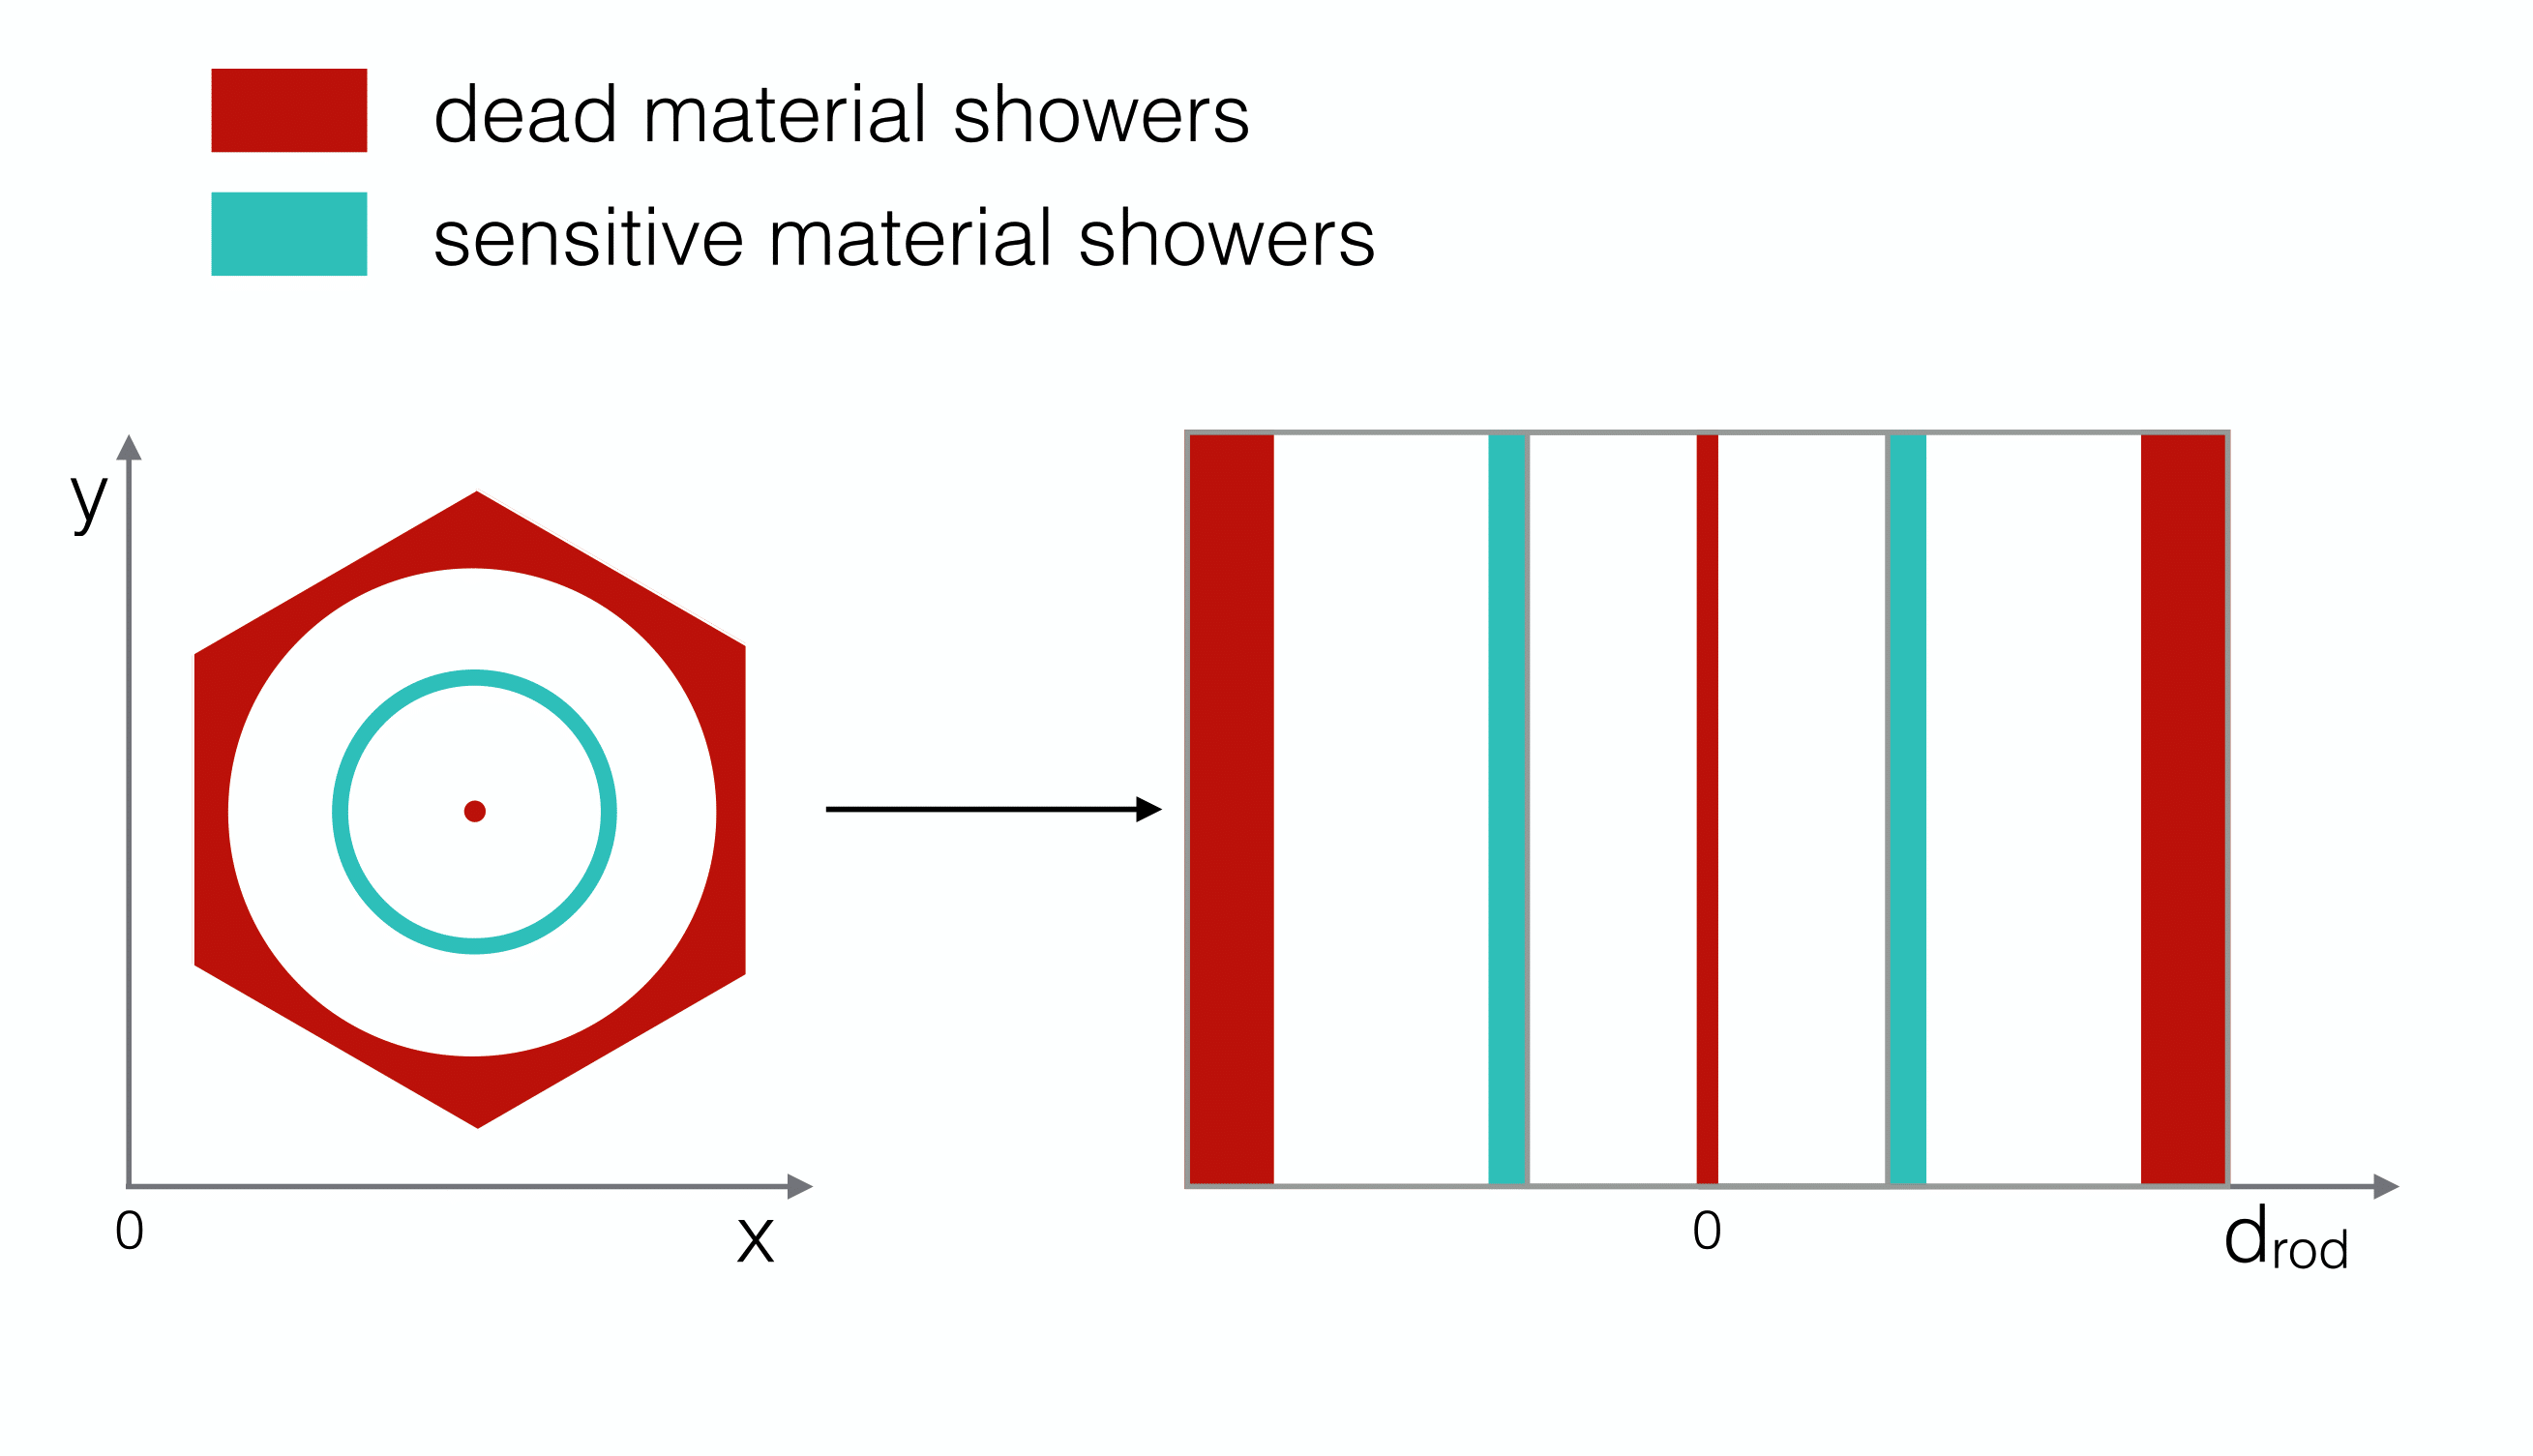
\includegraphics[width=0.8\textwidth]{MC/FirstClassifierData.png}
\caption{Schematic representation of preselected data for a first classifier in x vs y plane and distance plane. Electrons, created near rod center and on the borders of the module have low probablity to cross the sensitive material, while oppositely all of the electrons created inside liquid argon gap are sensitive material showers.}
\label{fig:SchemePresel}}
\end{figure}

\subsubsection{Second classifier}

\begin{figure}[!tbp]
\begin{minipage}[h]{0.49\linewidth}
\center{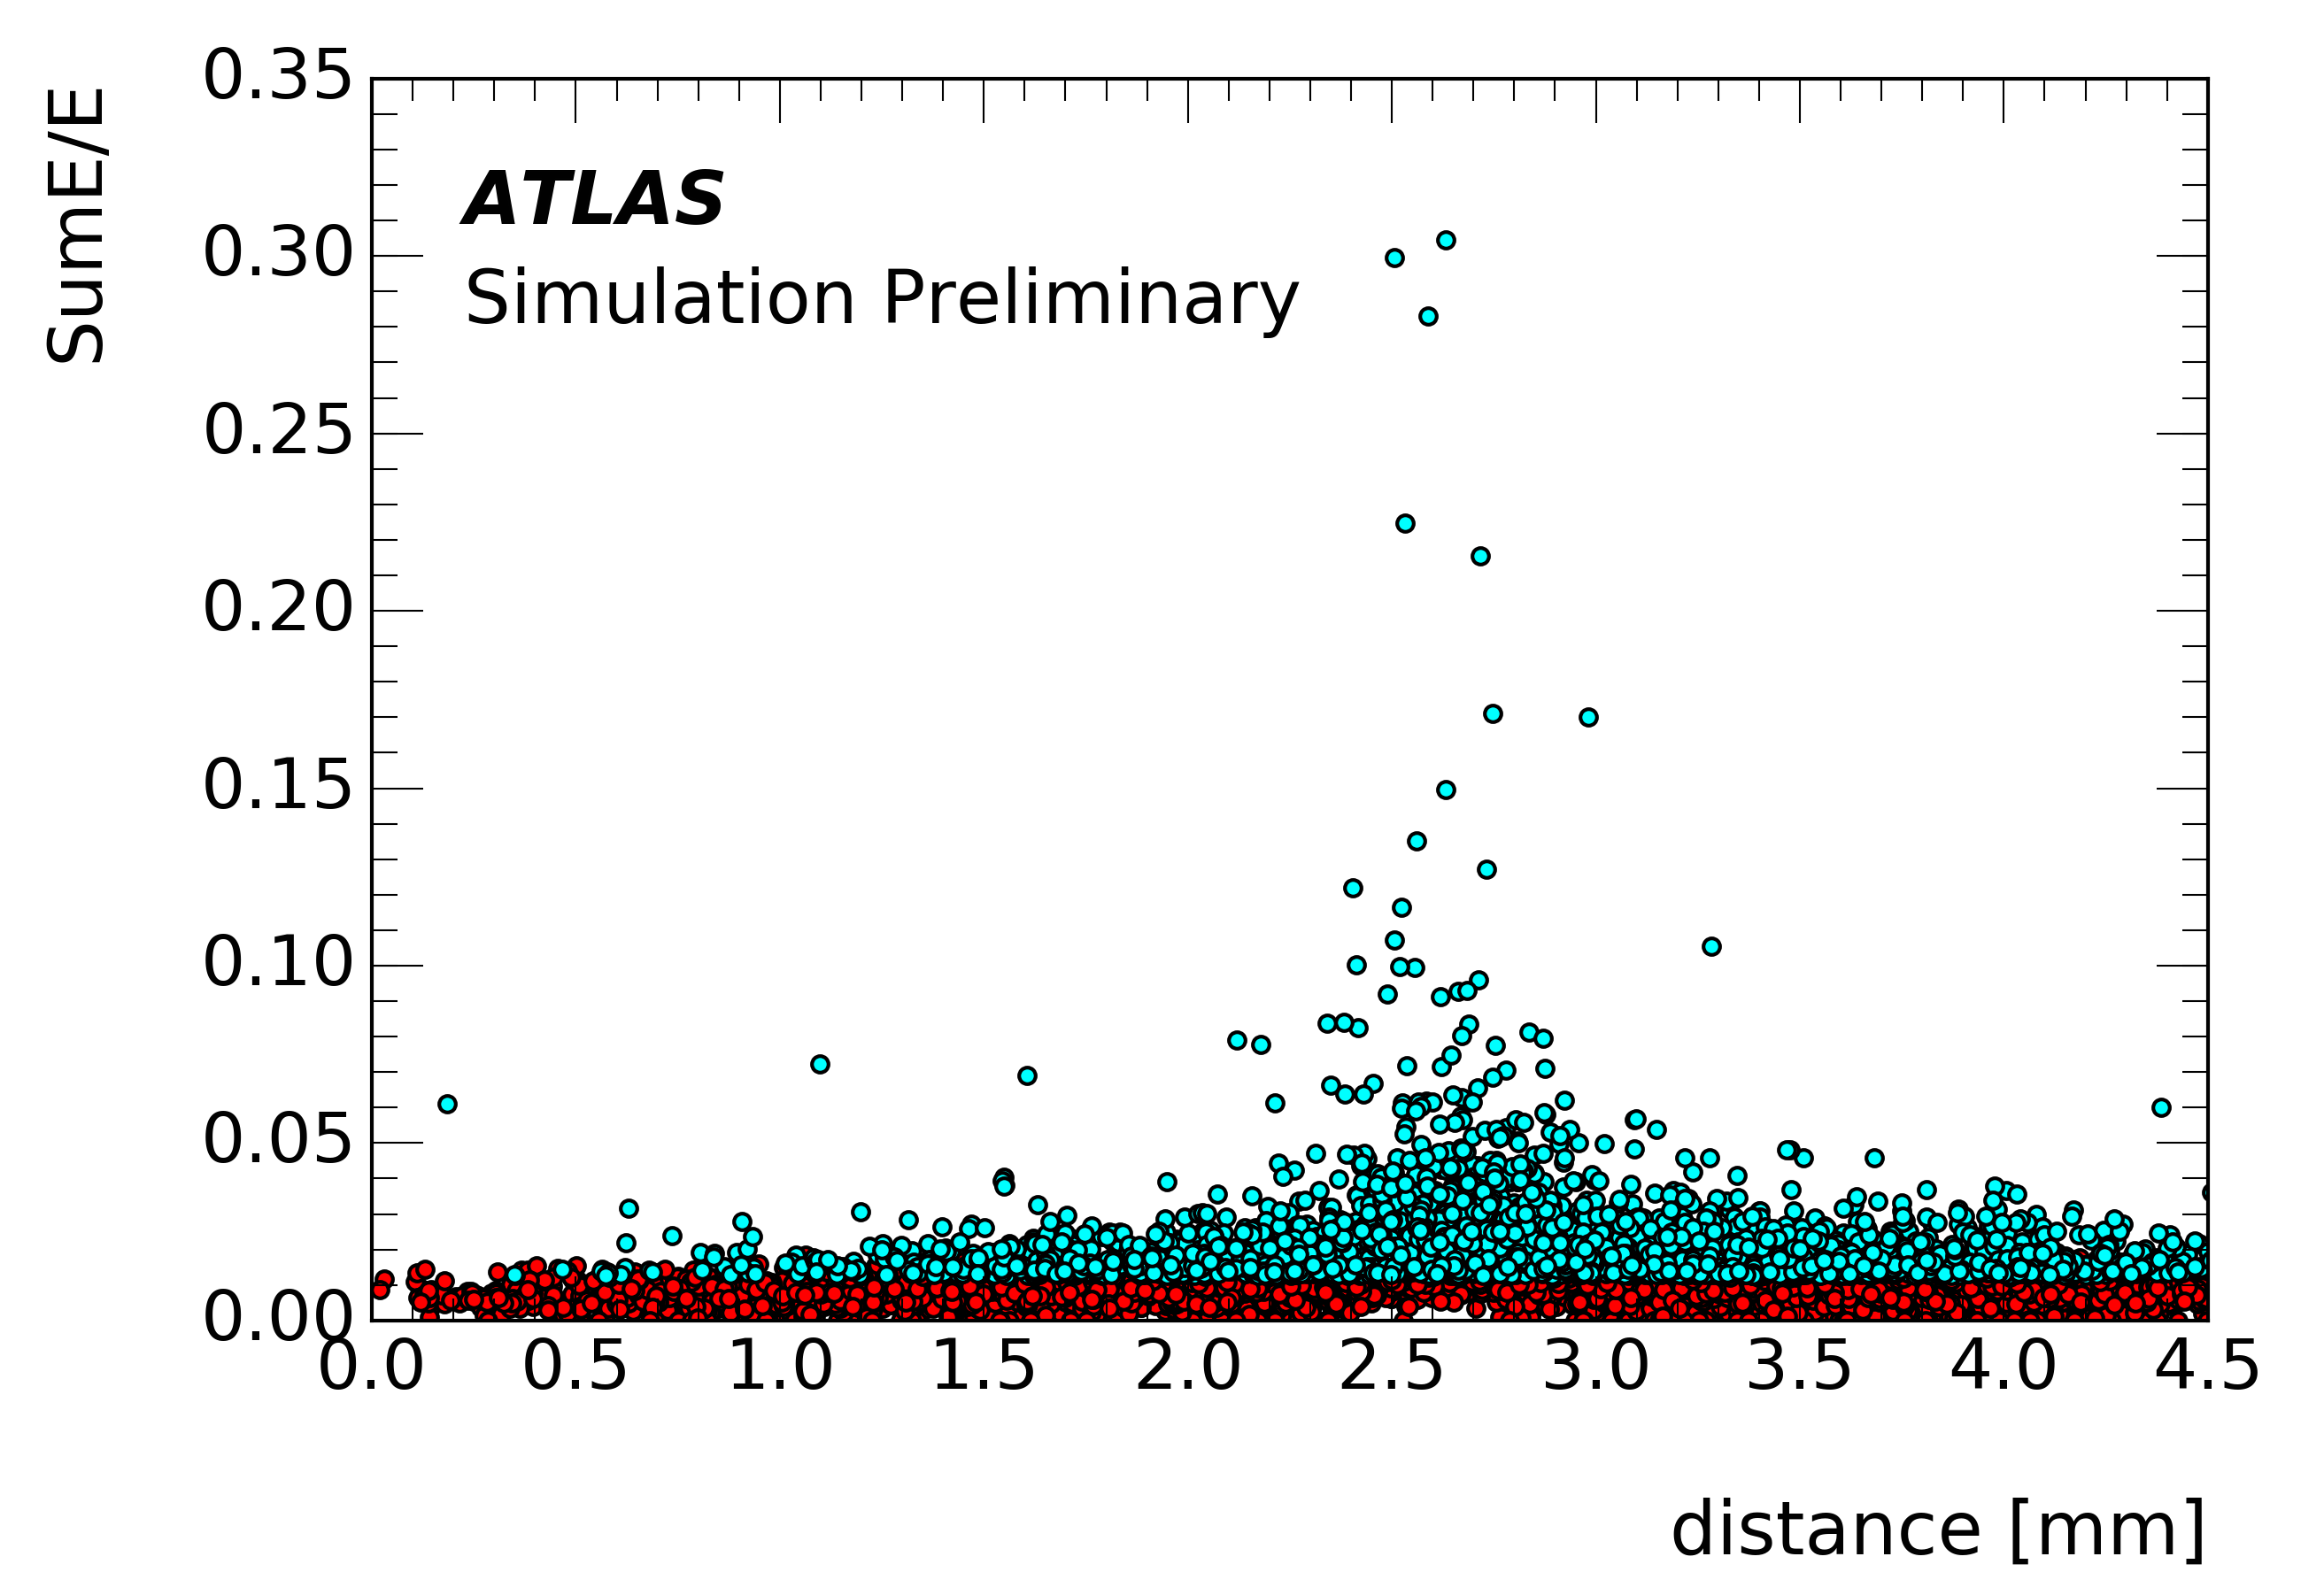
\includegraphics[width=1.\linewidth]{MC/firstClassifier.png} \\ a)}
\end{minipage}
\hfill
\begin{minipage}[h]{0.49\linewidth}
\center{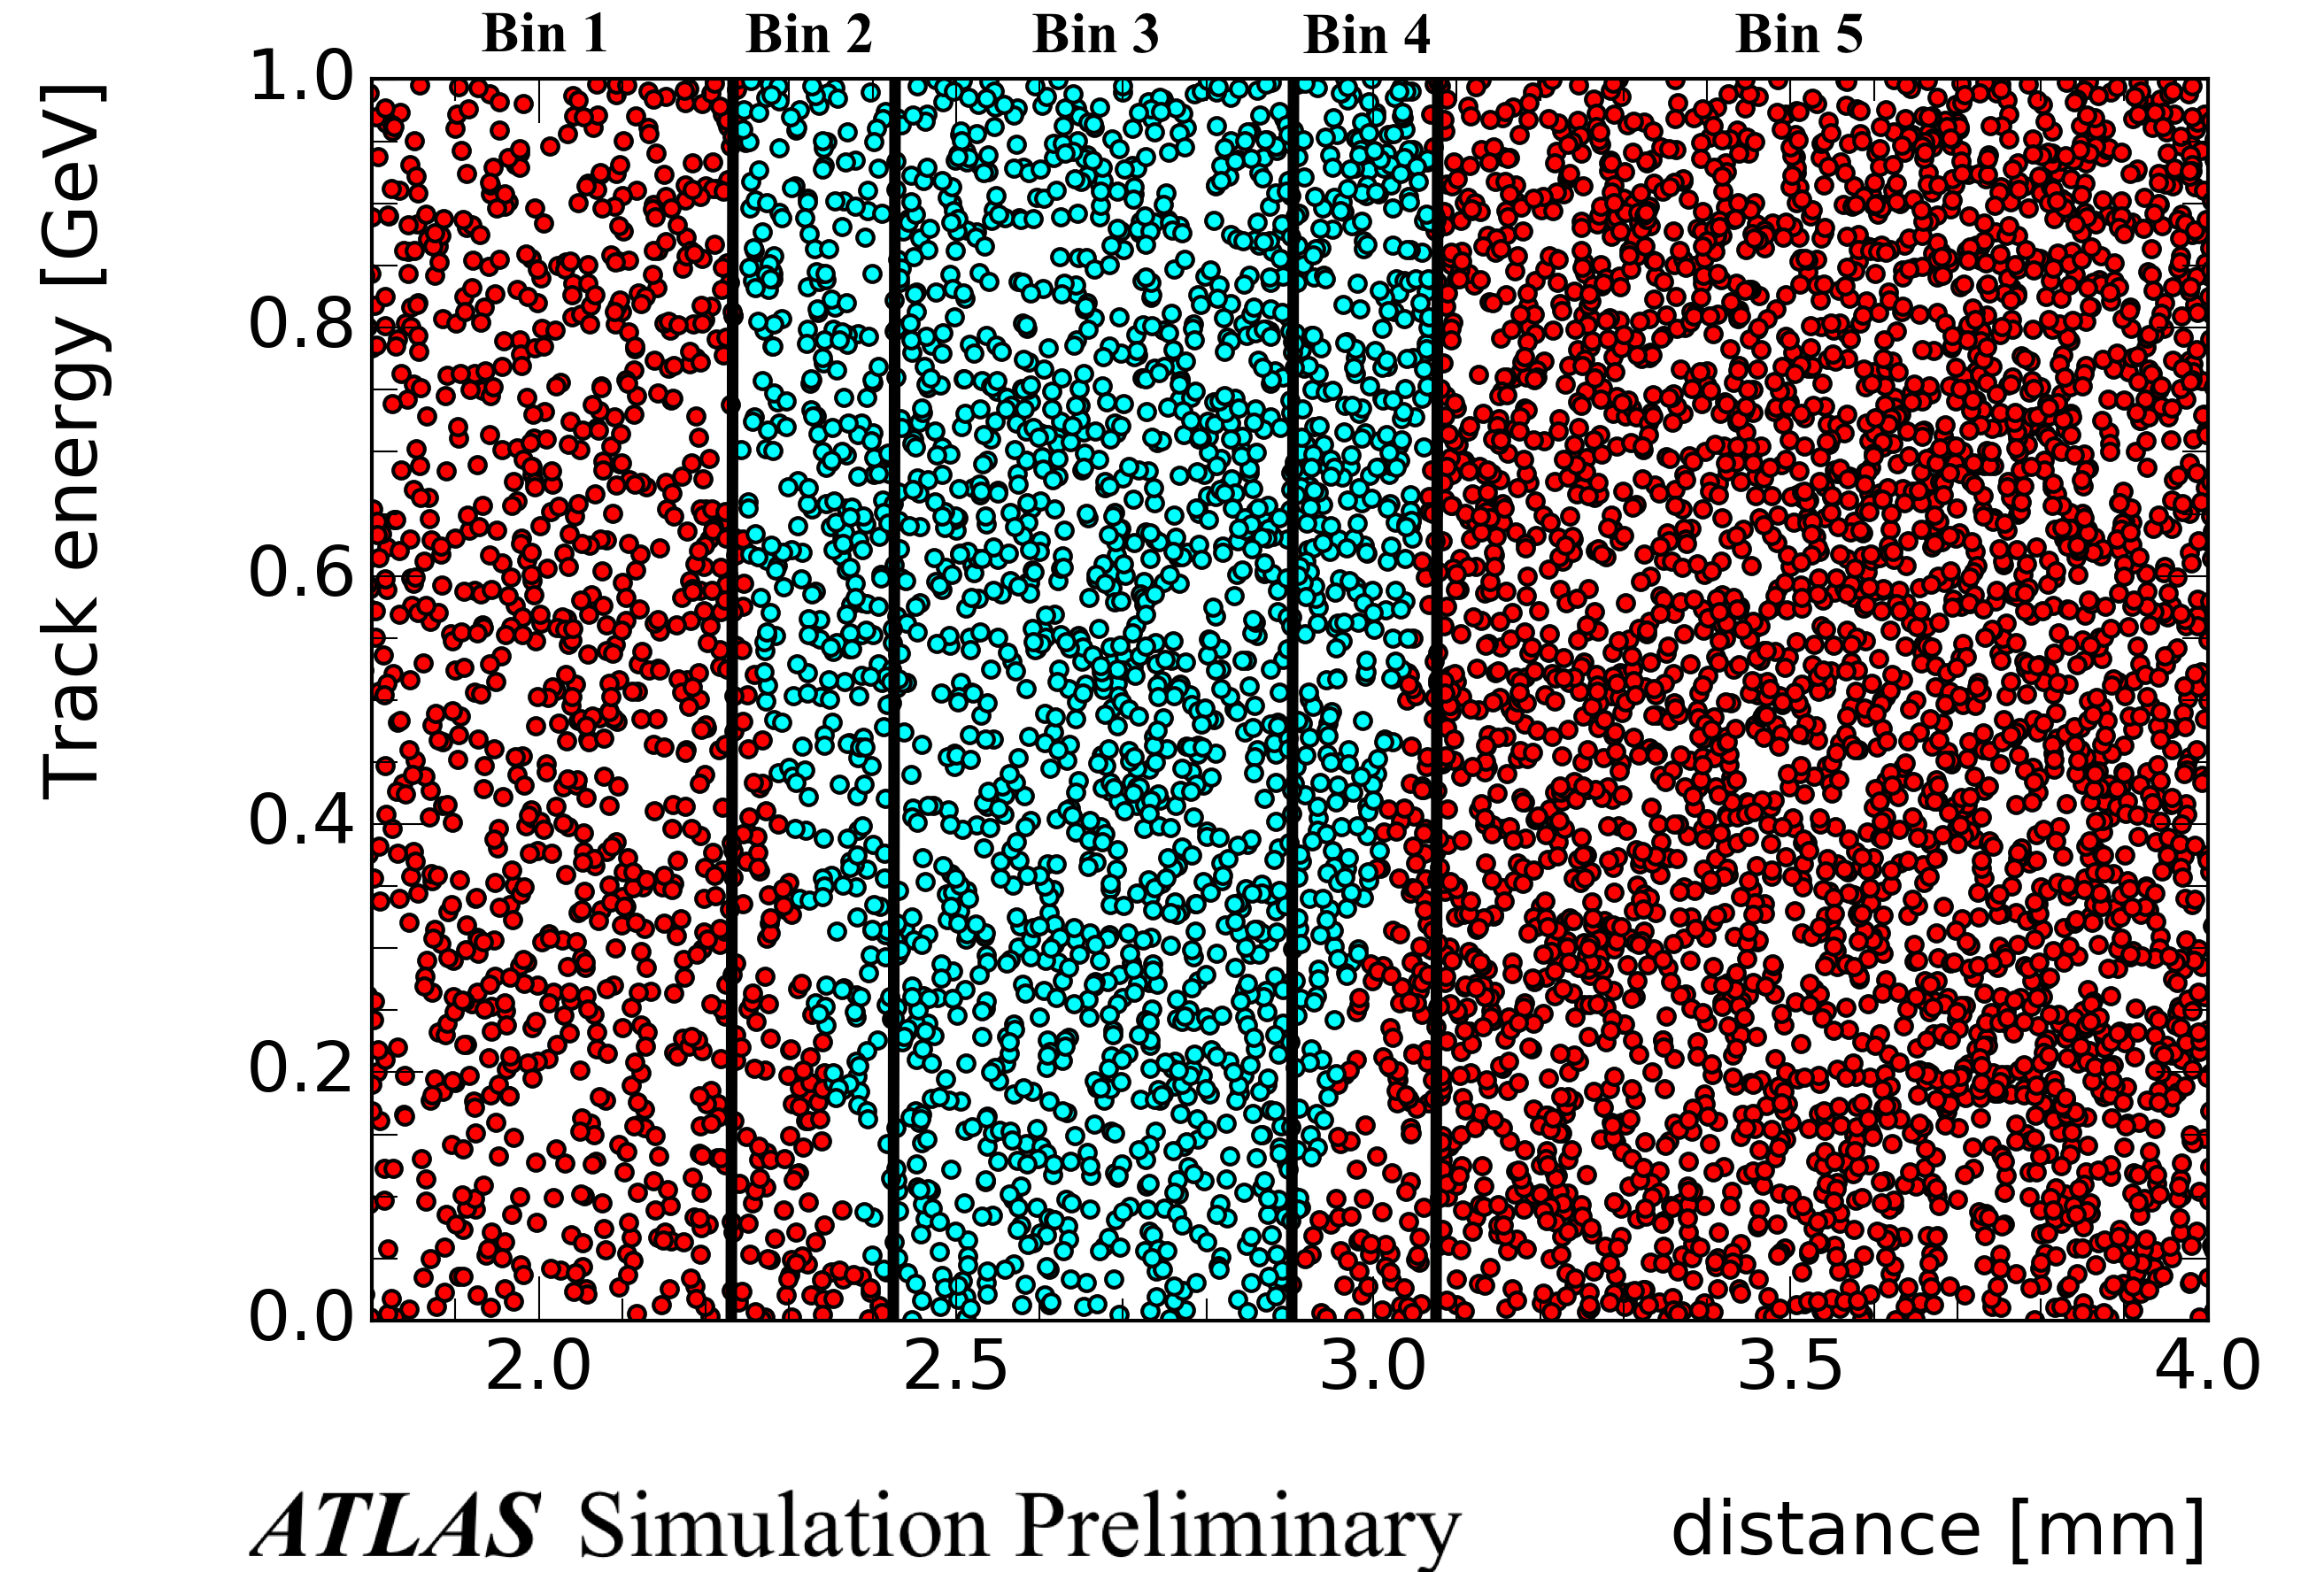
\includegraphics[width=1.\linewidth]{MC/secondClassifier.png} \\ b)}
\end{minipage}
\caption{Results of machine learning for a) first classifier b) second classifier. Cyan dots are corresponding to sensitive material showers, red - dead material showers. Black lines in Fig. b are corresponding to a resulting bin positions}
\label{fig:Class}
\end{figure}

Second classifier uses predictions of the first classifier as an input label. It is trying to reconstuct a best dividing hyperplane between two methods using a support vector machines. It uses as an input truth parameters of the electron, e.g. energy of the initial electron and its distance to a closest rod center. Different kernels have been tested and the best predictions have been obtained using RBF kernel (Eq. \ref{eq:RBF}).  Assuming, that $\eta^{momentum} \approx \eta^{position}$ classification is performed in each $\eta^{distance}$ bin used in a library. Example of the classifier output is shown in a Fig. \ref{fig:Class} b). As it is expected from the model, gap position is getting wider with higher energies of the electron.  Variation of the obtained parameters have been found small, so the mean of the parameters have been used.  

\subsubsection{Interpretation of results}

Because a full new regeneration of libraries and validation on a reconstructed variables is an a time-consuming procedure, the toy Monte-Carlo method have been developed for a cross-check of a classifiers and its interpretation. It uses pseudorapidity $\eta^{position}$, energy of electron and distance to a closest rod center from a data as a reference for a random generator. This simulation allows to compare shower energies and shower energy divided by  the energy of initial electron (SumE/E) distributions with and distributions from a full simulation, that are considered as a reference.

Several interpretations of the bin positions have been tested and the best one is showed in Fig. ~\ref{fig:Class} b) by a black lines. It was decided to make 3 bins corresponding to a liquid argon position instead of the only one. One contains, according to a classifier just sensitive material showers events, while in other 2 there is a mixture of dead material and sensitive material showers. The obtained positions of the liquid argon bins are wider, than a nominal ones, as expected from the model.
Comparison of SumE/E distributions using toy MC on old libraries (Fig. ~\ref{fig:Interpret} a) and the libraries with the new binning (Fig. ~\ref{fig:Interpret} b) have showed, that we could expect a better perfomance on a reconstructed values.


\begin{figure}[!tbp]
\begin{minipage}[h]{0.49\linewidth}
\center{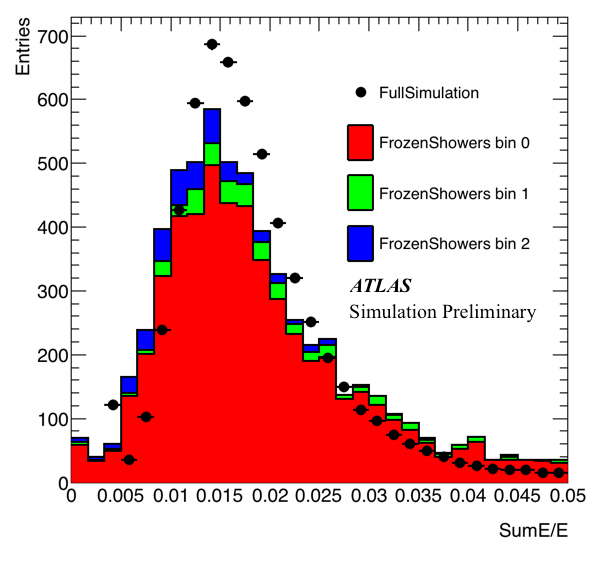
\includegraphics[width=1.\linewidth]{MC/oldSumE.png} \\ a)}
\end{minipage}
\hfill
\begin{minipage}[h]{0.49\linewidth}
\center{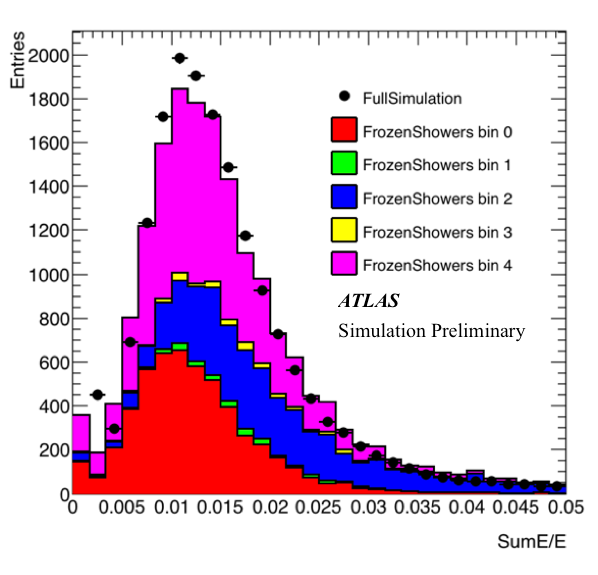
\includegraphics[width=1.\linewidth]{MC/newSumE.png} \\ b)}
\end{minipage}
\caption{Comparison of the distribtuions of shower energy divided by  the energy of initial electron between full simulation and toy MC using libraries for liquid argon gap bins and 2 closest to them bins for a) old "tuned" libraries with 1 liquid argon gap bin  b) new libraries binning with 3 liquid argon gap bins. There are still remaining differences between full simulation and toy MC, but new machine learning binning performs better.}
\label{fig:Interpret}
\end{figure}


\section{Validation of the new libraries}\label{sec:FSValidation}


Validation results for two different eta bins are shown on figure ~ a) and b). In a bin this new binning is performing better, than original one without any additional tuning. Unfortunately this is not true for all of the bins, as we can see on a figure ~ b). This eta bin have showed worst performance for a new binning, but it is performing still better, than original binning without tuning.

\begin{figure}[!tbp]
\begin{minipage}[h]{0.49\linewidth}
\center{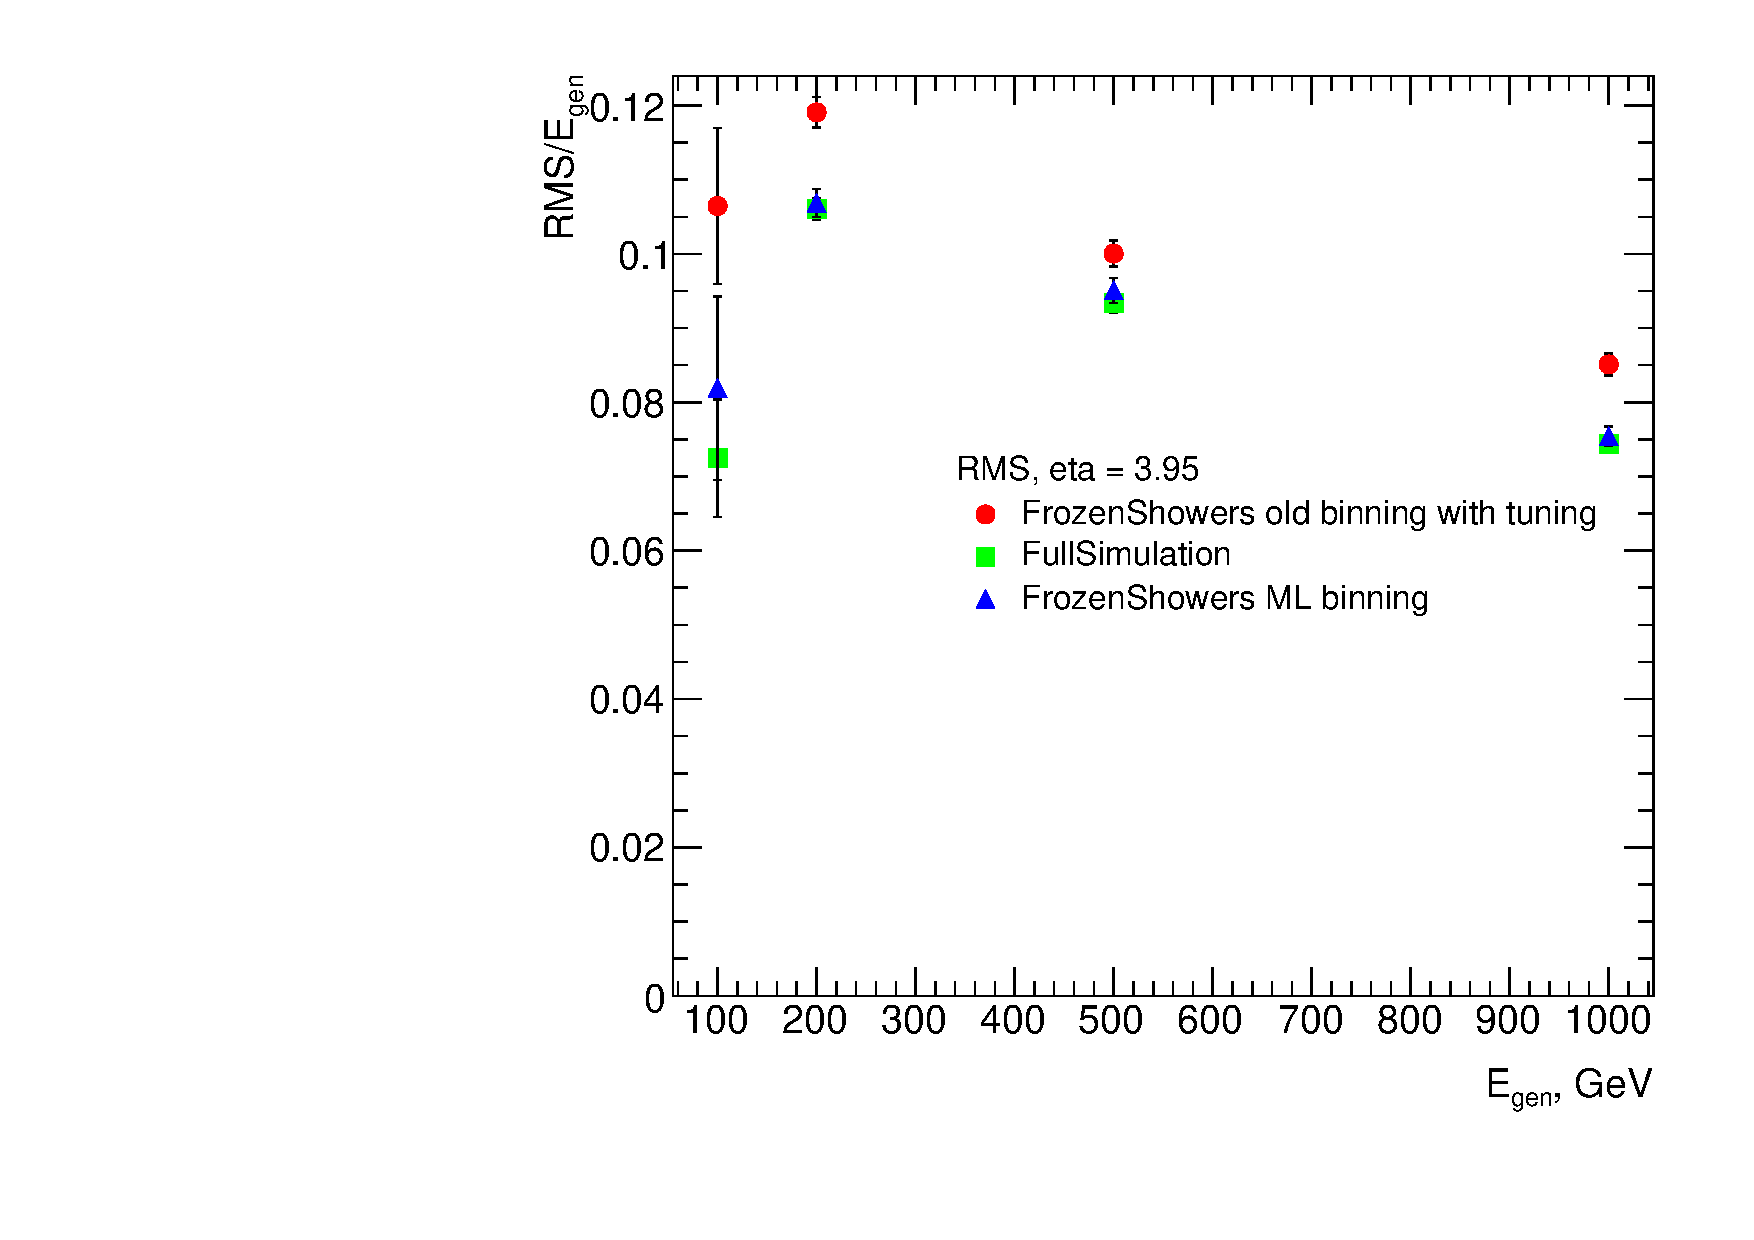
\includegraphics[width=1.\linewidth]{MC/rms3p95.pdf} \\ a)}
\end{minipage}
\hfill
\begin{minipage}[h]{0.49\linewidth}
\center{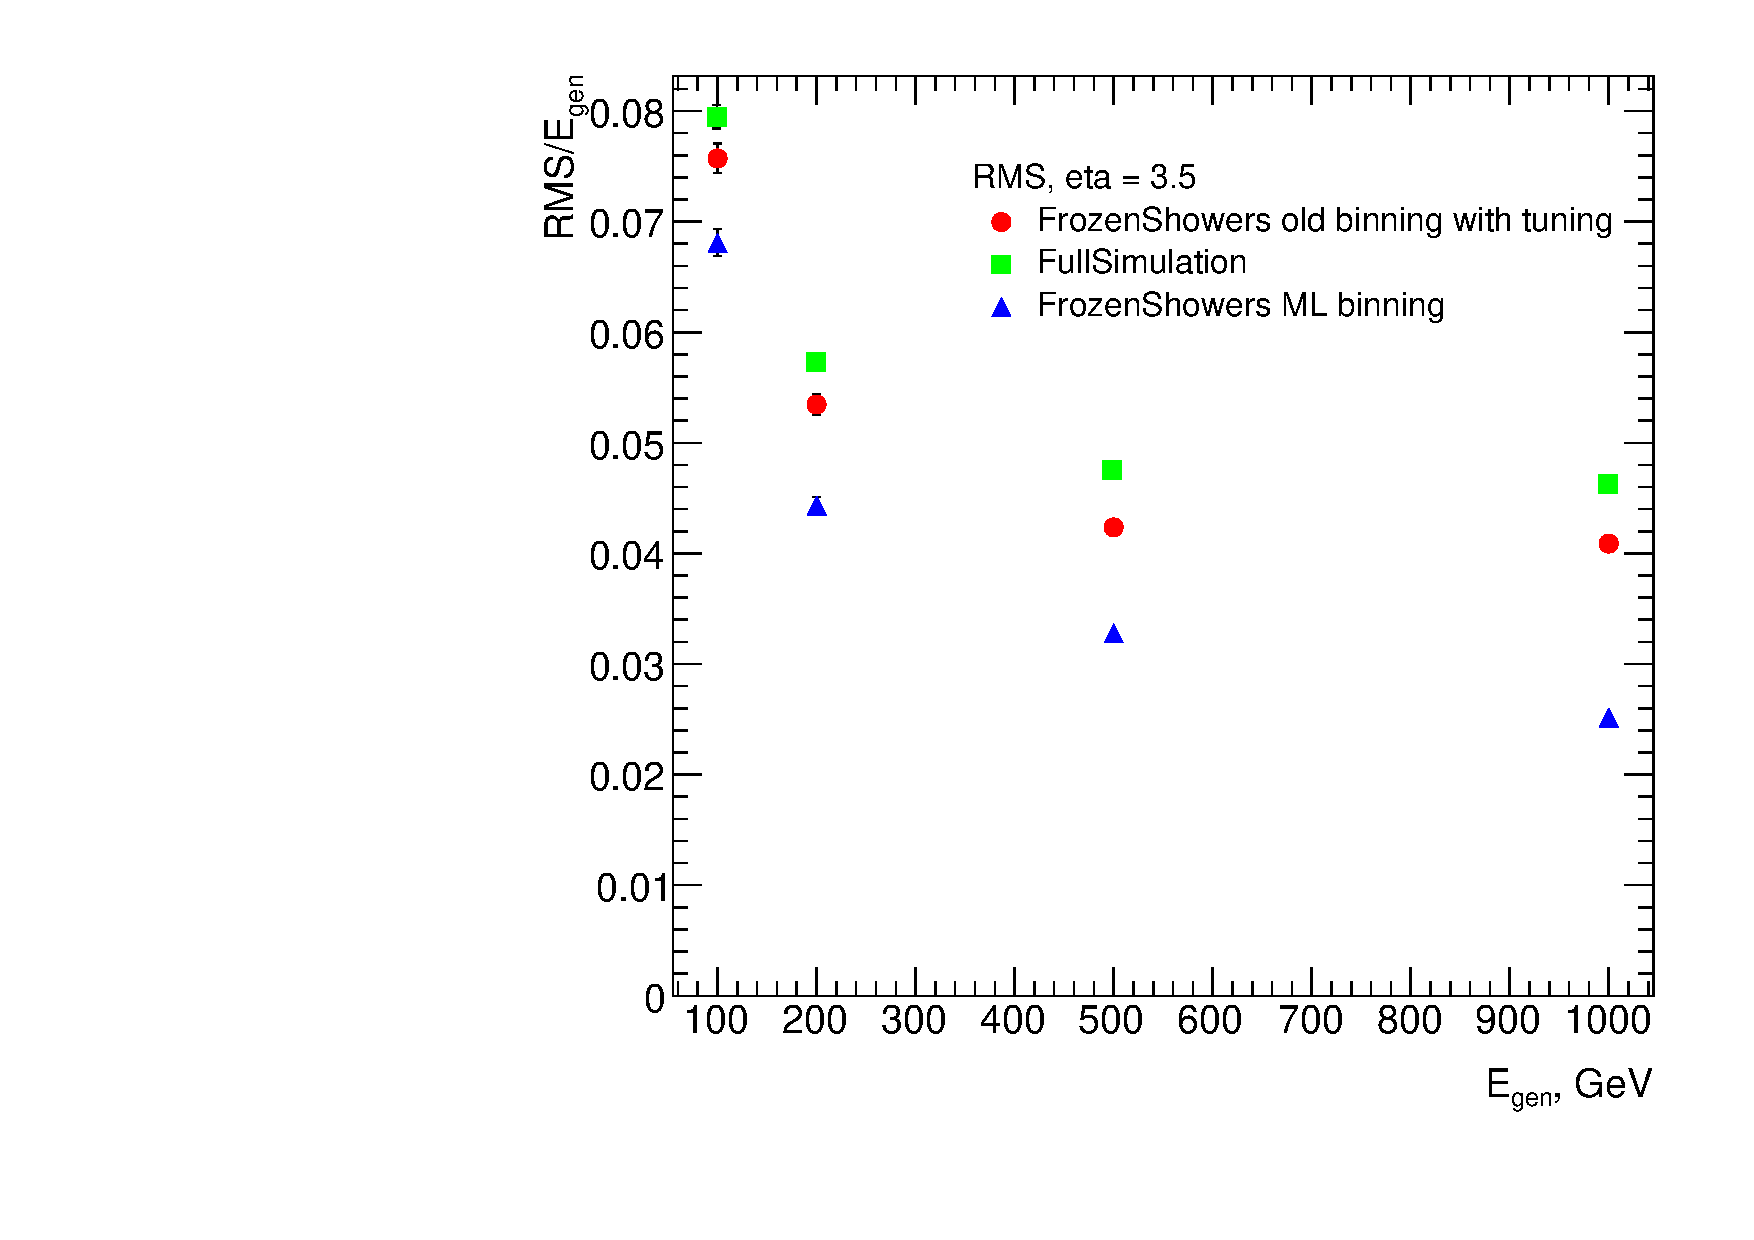
\includegraphics[width=1.\linewidth]{MC/rms3p5.pdf} \\ b)}
\end{minipage}
\caption{Resolution of reconstructed electrons for full simulation, new libraries with ML binning and old tuned libraries with original binning for a) eta =3.95 b)eta=3.5 }
\label{fig:Reso}
\end{figure}

\subsubsection{Validation on another objects}
\begin{figure}[!tbp]
\begin{minipage}[h]{0.49\linewidth}
\center{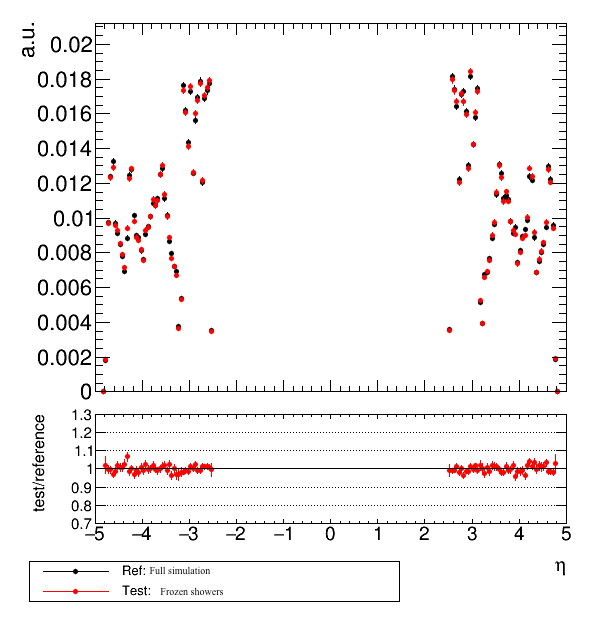
\includegraphics[width=1.\linewidth]{MC/Electron_Frwd_All_KinPlots_eta.png} \\ a)}
\end{minipage}
\hfill
\begin{minipage}[h]{0.49\linewidth}
\center{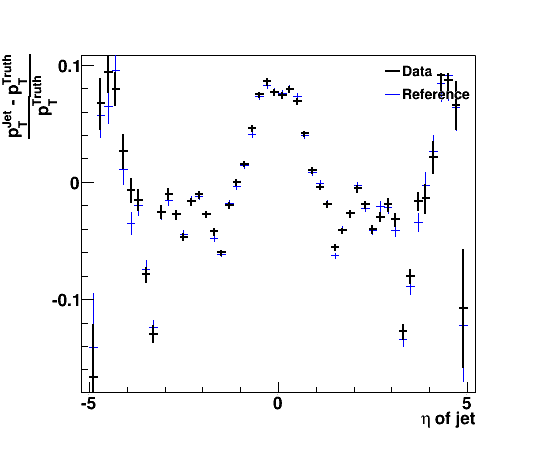
\includegraphics[width=1.\linewidth]{MC/erhResponseVsEta.png} \\ b)}
\end{minipage}
\caption{Resolution of reconstructed electrons for full simulation, new libraries with ML binning and old tuned libraries with original binning for a) eta =3.95 b)eta=3.5 }
\label{fig:OtherVal}
\end{figure}

This binning was used in a production of new libraries for Monte Carlo in a Run-2. It is planned to use more precise training sample for a future iterations of this procedure for improving performance of outlying eta bins.
